\documentclass[11pt,a4paper,twoside,openany]{tesis}
\usepackage{titlesec}
\usepackage{amsmath}
\usepackage{graphicx}
\usepackage[utf8]{inputenc}
\usepackage[spanish]{babel}
\usepackage[left=3cm,right=3cm,bottom=3.5cm,top=3.5cm]{geometry}
\usepackage{url}
\setcounter{secnumdepth}{3} % Para la numeración de las subsubsecciones
\usepackage{algorithm}
\usepackage{algpseudocode}
\usepackage{graphicx}
\usepackage{subcaption}
\usepackage{listings}
\usepackage{cite}
\setcounter{tocdepth}{3} 
\usepackage{titlesec}
\titlespacing*{\subsubsection}{0pt}{3.25ex plus 1ex minus .2ex}{1.5ex plus .2ex}
\titleformat{\subsubsection}[runin]{\normalfont\normalsize\bfseries}{\thesubsubsection}{1em}{} % Hace que el título sea inline
\usepackage{graphicx}  
\usepackage{float}     
\usepackage{setspace}
\onehalfspacing  % Interlineado de 1.5
\setlength{\parskip}{1em}
\usepackage{hyperref} % Para las citas clickeables 
\hypersetup{
    colorlinks=true,    
    linkcolor=blue,    
    citecolor=blue,     
    urlcolor=blue,      
    filecolor=blue
}
\usepackage{tocloft}
\setlength{\cftbeforesecskip}{0.5em}
\usepackage{enumitem}
\setlist[itemize]{topsep=3pt,itemsep=3pt,partopsep=0pt,parsep=0pt}

\usepackage{listings}
\usepackage{xcolor}

% Configuración de estilo para Python
\lstdefinestyle{pythonstyle}{
    language=Python,
    basicstyle=\ttfamily\small,
    keywordstyle=\color{blue},
    stringstyle=\color{red},
    commentstyle=\color{green!60!black},
    numbers=left,
    numberstyle=\tiny,
    frame=single,
    showstringspaces=false
}
\begin{document}

%%%% CARATULA

\def\autor{Carla de Erausquin}
\def\tituloTesis{Caracterización de trayectorias educativas a partir de producciones de código}
\def\runtitulo{Caracterización de trayectorias educativas a partir de producciones de código}
\def\runtitle{Characterization of educational trajectories based on Code Productions}
\def\director{Matías López y Rosenfeld}
\def\codirector{Pablo Turjanski}
\def\lugar{Buenos Aires, 2024}
\newcommand{\HRule}{\rule{\linewidth}{0.2mm}}
%
\thispagestyle{empty}

\begin{center}\leavevmode

\vspace{-2cm}

\begin{tabular}{l}

\includegraphics[width=2.6cm]{logofcen.pdf}
\end{tabular}


{\large \sc Universidad de Buenos Aires

Facultad de Ciencias Exactas y Naturales}

\vspace{7.0cm}

%\vspace{3.0cm}
%{
%\Large \color{red}
%\begin{tabular}{|p{2cm}cp{2cm}|}
%\hline
%& Pre-Final Version: \today &\\
%\hline
%\end{tabular}
%}
%\vspace{2.5cm}

\begin{huge}
\textbf{\tituloTesis}
\end{huge}

\vspace{2cm}

{\large Tesis de Licenciatura en Ciencias de Datos}

\vspace{2cm}

{\Large \autor}

\end{center}

\vfill

{\large

{Director: \director}

\vspace{.2cm}

{Codirector: \codirector}

\vspace{.2cm}

\lugar
}

\newpage\thispagestyle{empty}


%%%% ABSTRACTS, AGRADECIMIENTOS Y DEDICATORIA
\frontmatter
\pagestyle{empty}
%\begin{center}
%\large \bf \runtitulo
%\end{center}
%\vspace{1cm}
\chapter*{\runtitulo}

\noindent Con el creciente interés en la Ciencia y la Tecnología en los últimos años, los docentes enfrentan el desafío de corregir grandes volúmenes de código sin perder de vista el nivel de conocimiento alcanzado por los diferentes grupos de estudiantes. En este contexto, contar con herramientas que permitan predecir de manera temprana el riesgo de abandono en cursos introductorios de programación se vuelve crucial para enfocar la atención en aquellos alumnos que más lo necesitan.

\bigskip

\noindent\textbf{Palabras clave:} Clustering, CodeBERT, Embeddings, Enseñanza, Python, Programación.

\cleardoublepage
%\begin{center}
%\large \bf \runtitle
%\end{center}
%\vspace{1cm}
\chapter*{\runtitulo}
\noindent With the growing interest in Science and Technology in recent years, teachers face the challenge of correcting large volumes of code while keeping track of the knowledge level achieved by different groups of students. In this context, having tools that allow early prediction of dropout risk in introductory programming courses becomes crucial to focus attention on those students who need it most.

For this purpose, a dataset corresponding to an Introduction to Python Programming course was analyzed. Only their code productions were studied, transformed into embeddings with the help of the \emph{CodeBERT} model. Using dimensionality reduction techniques and, subsequently, clustering, it was possible to characterize some of the students who would drop out of the course early. In particular, the group of students who would abandon the course upon reaching the first evaluation instance. For the proposed exercises, it was not possible to differentiate between those students who would complete the course and those who continued with submissions beyond the first exam.
\bigskip

\noindent\textbf{Keywords:} Clustering, CodeBERT, Embeddings, Teaching, Python, Programming. % OPCIONAL: comentar si no se quiere

\cleardoublepage
\chapter*{Agradecimientos}

\noindent A Matías y Pablo por guiarme y enseñarme a lo largo de este proyecto y a quienes pude consultar y recurrir constantemente. 

\noindent A Mariano por acompañarme incondicionalmente a lo largo de mi carrera. 
 % OPCIONAL: comentar si no se quiere

\cleardoublepage
\hfill \textit{A mi papá, Claudio Francisco}
  % OPCIONAL: comentar si no se quiere

\cleardoublepage
\tableofcontents

\mainmatter
\pagestyle{headings}

%%%% ACA VA EL CONTENIDO DE LA TESIS

\chapter{Introducción}
\section{Motivación}

La programación, de manera directa e indirecta, forma parte de la vida cotidiana, y cada día aumenta su influencia. Su estudio constituye un aspecto central para la innovación en los procesos de enseñanza y aprendizaje en contextos de educación formal e informal. Además de ser una herramienta clave para el futuro, también es de vital importancia para la construcción de ciudadanía en un mundo atravesado por la tecnología. 

Esto fue reflejado por el Consejo Federal de Educación cuando definió que se lleven a cabo las acciones necesarias para que se incorpore la enseñanza de la programación en la escolaridad obligatoria \emph{con el fin de fortalecer el desarrollo económico y social de nuestro país}~\cite{resolucionProgramar}.

En particular, dentro de la Facultad de Ciencias Exactas y Naturales de la Universidad de Buenos Aires, la cantidad de alumnos que se inscriben a carreras afines a la programación, como lo es la Carrera en Ciencias de Datos, está en constante crecimiento: 

\begin{figure}[H]
    \centering
    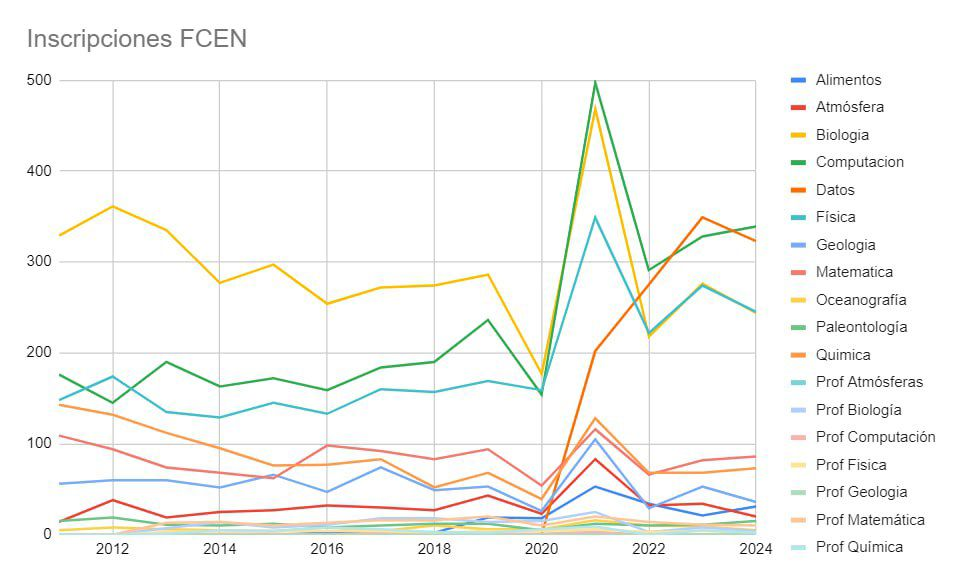
\includegraphics[width=0.8\textwidth]{imagenes/inscriptos-por-carrera.jpg}
    \caption{Número de inscriptos por carrera en la FCEN - UBA ~\cite{DOV}}
\end{figure}

En 2021, primera cohorte de inscripciones, alrededor de 300 personas se anotaron para comenzar sus estudios. En 2023, se anotaron más de 450 personas, a las cuales les correspondería cursar Introducción a la Programación en su primer año de carrera~\cite{primeros-datos}. Es entonces con este incremento en el alumnado que nace la necesidad de poder corregir código de manera rápida y eficiente. 

En un análisis exploratorio realizado por alumnos de la facultad basado en Censos de la UBA, Encuestas Docentes y el Sistema de Inscripciones, se observó que hay indicativos de que la deserción esté relacionada con el rendimiento del alumno en estas primeras materias ~\cite{analisis-exploratorio}. Por ello, consideramos importante la temprana detección de grupos más proclives a abandonar los cursos en cuestión. 

\section{CodeBert}

Se trata de un modelo preentrenado diseñado para entender y generar tanto lenguaje natural (NL) como lenguajes de programación (PL). Se basa en una arquitectura \emph{Transformer}, similar a \emph{BERT} y \emph{RoBERTa}, y fue entrenado usando datos bimodales (pares NL-PL) y unimodales (código o texto sin parejas), en seis lenguajes de programación (Python, Java, JavaScript, PHP, Ruby y Go) usando datos de repositorios públicos en GitHub. Esto último es particularmente relevante siendo que los cursos mencionados en la sección anterior, son dictados en el lenguaje Python.  . 

Este genera  \emph{embeddings} o representaciones vectoriales de fragmentos de código mediante su arquitectura basada en \emph{Transformers}. Al alimentar un fragmento de código como entrada, \emph{CodeBERT} convierte el código en una secuencia de \emph{tokens}, que luego procesa a través de sus capas para producir una representación contextualizada para cada \emph{token}. Estas representaciones capturan tanto la sintaxis como la semántica del programa.

El \emph{embedding} final para un fragmento completo puede obtenerse utilizando el vector asociado al \emph{token} especial [CLS], que representa el significado agregado de la secuencia. Estos \emph{embeddings} pueden emplearse para tareas como búsqueda de código, clasificación, o generación de documentación, ya que contienen información relevante tanto del contenido del código como de su contexto.

\emph{CodeBERT} demostró un rendimiento sobresaliente en tareas de búsqueda de código y generación de documentación en comparación con modelos preentrenados solo en lenguaje natural o código~\cite{codeBert}. Esto, sumado al público y fácil acceso del modelo~\cite{codeBert-repo} , hicieron que se optara por él para el análisis de este trabajo.

\section{CodeBert y el ámbito estudiantil}

En los últimos años se observaron muchos esfuerzos en desarrollar herramientas para la enseñanza de la programación que pudieran capturar las características individuales para potenciar el aprendizaje. Algunas de estas líneas han buscado usar la noción de similitud como cantidad de cambios a realizar en un código para proponer corregir errores en ejercicios de manera automática~\cite{gulwani2018automated}.

Gracias a los avances tecnológicos previamente mencionados, es posible trabajar con \emph{embeddings} de manera \emph{más sencilla} y poder proyectar texto en un espacio multidimensional. Una aplicación fue capturar semejanzas entre entregas de estudiantes y, organizándolas en orden por similitud, facilitar la tarea de corrección~\cite{simgrade}. Además, este tipo de análisis sirve para identificar el conocimiento adquirido en temas específicos de un curso~\cite{brigante2020evaluation} como la evolución a lo largo del mismo~\cite{wu2018zeroshotlearningcode}. Esto abre la oportunidad para poder planificar intervenciones docentes en momentos tempranos que potencien el aprendizaje, que en cursos masivos antes resultaba imposible. 

En su investigación usando \emph{code2vec},  Brigante  evaluó si el código fuente en sí mismo, sin ejecutar el código o evaluar su salida, era suficiente para estimar la calidad de las respuestas de los estudiantes. Los resultados sugieren que, aunque no siempre se alcanzaron los resultados esperados, el análisis del código fuente ofrece algunos indicios útiles para evaluar la calidad del desarrollo del estudiante ~\cite{brigante2020evaluation}.

\section{Propuesta}

Utilizando el modelo \emph{CodeBERT}, proponemos caracterizar la trayectoria académica de los estudiantes de un curso introductorio de programación, basándonos exclusivamente en sus producciones de código. Esto puede ser particularmente útil para los docentes, ya que permite identificar a los grupos más vulnerables en la cursada y saber en cuáles concentrar sus esfuerzos.

%% ...
\chapter{Materiales y métodos}
\section{Fuentes de datos}
Los datos empleados para este análisis son el resultado de entregas de alumnos de la materia Programación en Python de la UNSAM, dictada de manera virtual en contexto de pandemia.  La materia contó con más de 1200 preinscriptos, incluyendo  un  40\%  de  personas  que  residen  fuera  del  Área  Metropolitana de Buenos Aires (AMBA).

Este se dictó con el objeto de ~\emph{enseñar los fundamentos del lenguaje Python orientado al manejo de datos, a la escritura de scripts y a una organización adecuada de los programas; enseñar  algunos  rudimentos  de  la  teoría  de  algoritmos,  incluyendo  conceptos  básicos  de  la teoría de la complejidad y algunas estructuras de datos no triviales; e introducir la programación orientada a objetos} ~\cite{unsam2020}.

Con un total de 12 unidades y una duración de 3 meses, se realizó una evaluación permanente con entregas semanales de entre cuatro y seis ejercicios obligatorios por semana; llegando en total a  56  ejercicios  seleccionados  a  lo  largo  de  todo  el  curso.  Además  de  evaluar  estas  entregas semanales, se tomaron dos exámenes parciales de forma virtual y sincrónica con modalidad de opción múltiple lo que permitió una corrección automatizada. Si bien contamos con los datos sobre los resultados de la evaluación de este curso, no fueron considerados ya que se realizó foco en predecir quienes sencillamente lo habían finalizado. Para aprobar la materia resultó necesario haber realizado adecuadamente el 70\% de los  ejercicios  obligatorios  y  haber  aprobado  ambos  exámenes  parciales ~\cite{unsam2020}.


\subsection{Proceso ETL de los datos}

\subsubsection{Extracción}\textbf{ }

Los datos se extrajeron a partir de de un google drive \textcolor{red}{charlar con matias}

De las 12 unidades que constituyeron al curso, para este análisis se tuvieron en cuenta únicamente las primeras 5. Al finalizar la unidad 4 fue la presentación del primer examen. Siendo deseable la caracterización temprana de aquellos estudiantes que abandonarán el programa y con intenciones de que esto pueda replicarse en cursos futuros, se consideró estudiar únicamente la primera mitad del mismo. 

A continuación se detallan los contenidos de las primeras unidades a analizar:

\begin{figure}[H]
    \centering
    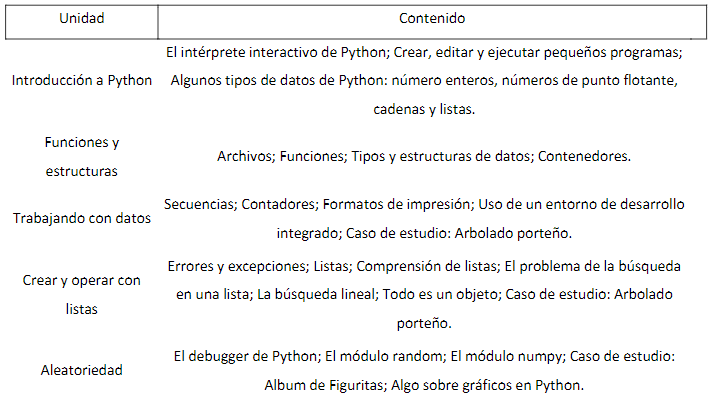
\includegraphics[width=0.8\textwidth]{imagenes/modulos-curso.PNG}
    \caption{Contenidos evaluados en las unidades extraídas para este análisis ~\cite{unsam2020}}
\end{figure}

A los códigos extraídos de los 31 ejercicios comprendidos por estas unidades para los más de 800 alumnos de los cuales los obtuvimos, se los anonimizó. Para ello asociamos cada entrega con un identificador creado por nosotros, \emph{id\_anon}.

Se obtuvieron entonces en una primera instancia tres conjuntos de datos: 
\begin{itemize}
    \item \textbf{Anonimizador} que describe por entrada, para cada identificador, el identificador propio del ejercicio en cuestión, el nombre del archivo y la fecha y hora de entrega. Esto último es particularmente útil siendo que los alumnos podían realizar más de una entrega del mismo ejercicio.
    \item \textbf{Código} archivos \emph{.py} con los ejercicios con el mismo nombre que en la tabla anterior. Los nombres eran identificadores unívocos de los ejercicios lo que permitía vincularlos con el Anonimizador.
    \item \textbf{Resultados} de la cursada, con el identificador del estudiante, la nota de las entregas, los dos parciales y el trabajo práctico y un booleano haciendo referencia a si este aprobó o no la cursada. Dentro de este conjunto se encuentran únicamente aquellos alumnos que finalizaron la materia.  
\end{itemize} 

\subsubsection{Transformación}\textbf{ }

Webster et al. definen \emph{token} como una unidad básica en el procesamiento del lenguaje natural (NLP) que no necesita ser descompuesta en etapas posteriores del procesamiento. Puede ser un elemento como una palabra, un modismo o una expresión fija, que se trata como un átomo indivisible para los propósitos de la computación. La tokenización implica identificar estas unidades básicas en el texto, que son esenciales para realizar análisis o generación de texto posteriores~\cite{tokens}.

El modelo de interés, \emph{CodeBERT}, tiene un límite de 512 \emph{tokens} para la entrada. Esto significa que cualquier secuencia de código a procesar tiene que ser truncada o dividida para que no exceda esta cantidad. Es debido a esta limitación del modelo que se tomó la decisión de realizar una limpieza del código, eliminando así los comentarios del mismo. Además, por ejercicio a entregar se contaba con una función \emph{objetivo}, que fue la que se consideró para la extracción. Cabe destacar que de realizarse testeos automatizados, aquellos archivos que no contaran con dichas funciones \emph{objetivo} (o estuvieran mal nomencladas), habrían fallado. Esto se consideró como un criterio adicional para discriminar entre qué datos incorporaríamos al análisis subsiguiente y cuáles no. 

\begin{figure}[H]
    \centering
    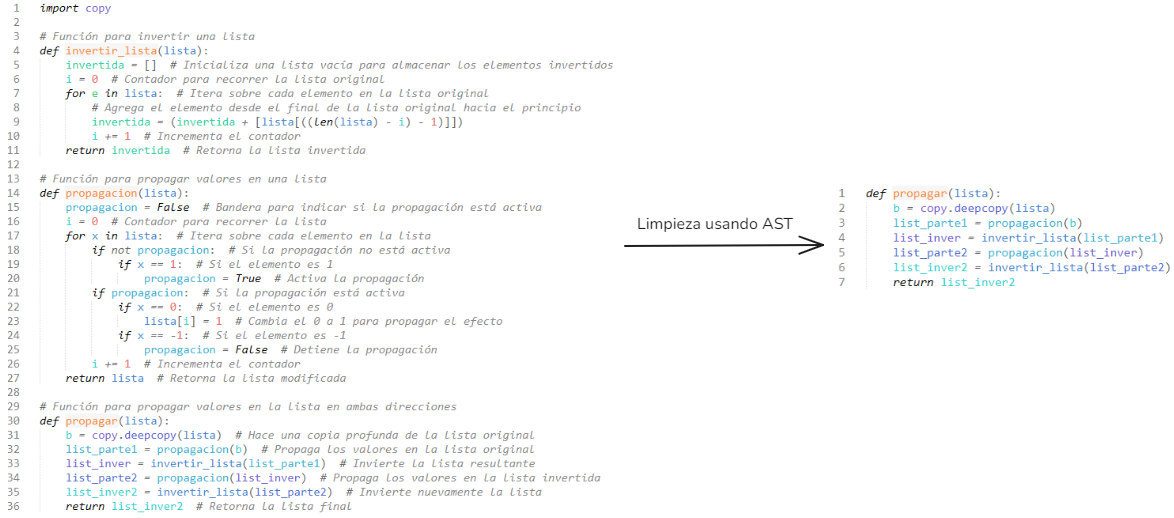
\includegraphics[width=1\textwidth]{imagenes/ast.PNG}
    \caption{Código entregado por un estudiante como resolución del ejercicio \emph{propagar} antes y después de su limpieza. A modo de ejemplo, utilizando \emph{nlkt.tokenize} la cantidad de \emph{tokens} del código de la izquierda es de 337 y el de la derecha, 38.}
\end{figure}

Mencionan Glassman et al. en su trabajo \emph{OverCode: visualizing variation in student solutions to programming problems at scale} \cite{overcode} en relación a la limpieza de comentarios de código a analizar que \emph{...la variación en los comentarios es tan grande que agruparlos y resumirlos requerirá un diseño adicional significativo}. Este es otro motivo para eliminar el texto adicional de las producciones de alumnos.

Para el código en sí, se hizo uso de los \emph{Abstract Syntax Trees (AST)}. Un árbol de sintaxis abstracta es una representación estructurada de un programa, que retiene la estructura esencial del árbol de análisis sintáctico pero elimina los nodos innecesarios. Mantiene la precedencia y el significado de las expresiones, simplificando la representación al omitir la mayoría de los nodos de los símbolos no terminales\cite{cooper2011engineering}. Esto permitió un rápido filtrado de las llamadas funciones \emph{objetivo} y la eliminación de los comentarios de manera mucho más eficiente que utilizando expresiones regulares. Para lo mencionado anteriormente puede utilizarse la biblioteca \emph{ast} \cite{ast} en Python.



\textbf{Código a embeddings}

Como se mencionó anteriormente, se usó el modelo \emph{CodeBERT} para pasar del código a los \emph{embeddings}. Desde la biblioteca \emph{transformers} \cite{roberta_model} es posible importar tanto el \emph{tokenizador} como el modelo en sí con:

\begin{lstlisting}[language=Python]
from transformers import RobertaTokenizer, RobertaModel
tokenizer = RobertaTokenizer.from_pretrained("microsoft/
codebert-base")
model = RobertaModel.from_pretrained("microsoft/codebert-base")
\end{lstlisting}

Luego, para cada archivo \emph{.py}, una vez limpiado como se mencionó en secciones anteriores, bastó con realizar lo siguiente para obtener sus \emph{embeddings} a partir de \emph{CodeBERT}:

\begin{algorithm}
\caption{Cálculo de Embeddings para Códigos}
\begin{algorithmic}[1]
\State Inicializar lista vacía \texttt{embeddings}
\For{cada \texttt{código} en la lista de códigos}
    \State \textbf{Intentar:}
        \State Tokenizar el \texttt{código}
        \State Crear secuencia de tokens:
        \State \hspace{\algorithmicindent} [CLS] + tokens\_código + [SEP] + [EOS]
        \State \hspace{\algorithmicindent} \textit{// CLS: token de inicio de secuencia}
        \State \hspace{\algorithmicindent} \textit{// SEP: token separador}
        \State \hspace{\algorithmicindent} \textit{// EOS: token de fin de secuencia}
        \State Convertir tokens a IDs
        \State Calcular embedding usando el modelo
        \State Añadir \{código, embedding\} a \texttt{embeddings}
    \State \textbf{Si hay error:}
        \State Imprimir mensaje de error
\EndFor
\end{algorithmic}
\end{algorithm}

Además, se almacenaron los \emph{embeddings} normalizados. La normalización de \emph{embeddings} ajusta los vectores para que tengan una magnitud uniforme, comúnmente de longitud 1. Esto facilita comparaciones y cálculos posteriores al eliminar diferencias en escalas. Para ello usamos la biblioteca \emph{normalize} de \emph{scikit-learn} \cite{sklearn_normalize}.

\subsubsection{Carga} \textbf{ }

Para almacenar los tres conjuntos de datos previamente mencionados, se optó por un tipo de base No-SQL, MongoDB que se creó localmente. Los motivos son varios:
\begin{itemize}
    \item \textbf{Flexibilidad en el esquema}: MongoDB, al ser una base de datos NoSQL, permite trabajar con un esquema flexible. Esto es especialmente útil en para este trabajo, ya que los datos presentan diferentes tipos y estructuras que pueden evolucionar con el tiempo. La flexibilidad de MongoDB permite la adaptación del modelo de datos sin necesidad de realizar cambios complejos en el esquema.
    
    \item \textbf{Facilidad de uso}: La sintaxis de MongoDB es sencilla e intuitiva, lo que simplifica su uso y permite concentrarse en el análisis y manipulación de los datos en lugar de en la configuración del entorno.
    
    \item \textbf{Documentación abundante}: MongoDB cuenta con una amplia documentación lo que facilitó mucho el trabajo con esta herramienta. 
    
    \item \textbf{Manejo eficiente de grandes volúmenes de datos}: Dado que MongoDB almacena los datos en formato BSON (una representación binaria de JSON), es capaz de manejar grandes volúmenes de datos de manera eficiente.
    
    \item \textbf{Capacidad de escalabilidad horizontal}: MongoDB permite la escalabilidad horizontal mediante la adición de nodos al clúster de base de datos. Esto es una ventaja importante si se prevé un crecimiento en el volumen de datos o en la demanda de las consultas. A sabiendas de que en un futuro podría agregarse información adicional por parte de los análisis posteriores, esto resulto particularmente útil \cite{MongoDB-docs}.
    
    \item \textbf{Integración con herramientas de análisis y desarrollo}: MongoDB se integra fácilmente con una amplia variedad de herramientas de análisis de datos, lenguajes de programación y bibliotecas, lo que facilita el desarrollo de aplicaciones y análisis de datos en entornos como Python. En particular, a la hora de implementar un conector para la base de datos creada localmente, se usó la biblioteca \emph{pymongo} \cite{pymongo}.
\end{itemize}

Luego, la base de datos en cuestión se organizó con la siguiente estructura de colecciones:

\begin{figure}[H]
    \centering
    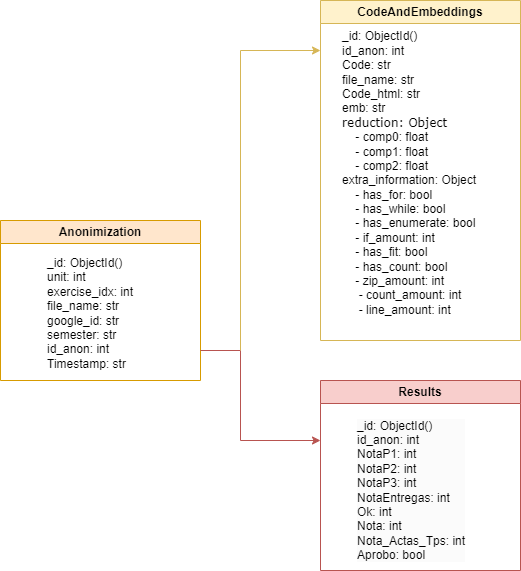
\includegraphics[width=0.5\textwidth]{imagenes/diagrama-base.png}
    \caption{Esquema del diseño de la base de datos.}
    \label{diagrama-base}
\end{figure}

Donde la mayoría de los campos en cuestión fueron explicados en secciones anteriores. En cuanto a la colección \textbf{CodeAndEmbeddings}, se ahondará más adelante en la información restante.

La base de datos para guardar todos los datos pertinentes a este estudio fue \emph{hosteada} localmente. Esta decisión resultó conveniente por varias razones: primero, permitió un acceso rápido y eficiente a los datos; segundo, facilitó el control total sobre la seguridad y la integridad de la información; y tercero, eliminó la dependencia de servicios externos, lo que mejoró la reproducibilidad del estudio.

Además, el \emph{hosting} local de la base de datos proporcionó flexibilidad para realizar consultas complejas y actualizaciones en tiempo real, lo que fue crucial para el análisis iterativo de los datos durante el desarrollo del proyecto.

\section{Etapas de trabajo para el Análisis de los Datos}

\subsection{Reducción de la dimensionalidad}

El análisis de componentes principales (PCA) es una técnica de reducción de dimensionalidad que transforma datos de alta dimensión en un espacio de menor dimensión, conservando la mayor parte de la varianza original. Para \emph{embeddings} como los de \emph{CodeBERT}, es posible usar PCA para reducir la dimensionalidad de los vectores, preservando la información relevante y facilitando su visualización y análisis\cite{pca-musil}.

PCA ofrece ventajas claras para \emph{embeddings}. Permite reducir los vectores a dos o tres dimensiones, permitiendo la detección de patrones en los datos \cite{pca-musil}. También ayuda a eliminar ruido y redundancias, mejorando la calidad del análisis posterior. Sin embargo, como señala Basirat \cite{pca-basirat}, tiene limitaciones con datos no normalmente distribuidos.

Otra desventaja es el costo computacional de calcular la matriz de covarianza, especialmente para grandes volúmenes de datos. Esto puede ser un obstáculo en proyectos extensos de, por ejemplo, procesamiento del lenguaje natural\cite{pca-basirat}. Sin embargo, esta sigue siendo una herramienta valiosa para la reducción de dimensionalidad y la optimización en el manejo de \emph{embeddings}, motivo por el cual se usó para los análisis posteriores.

Teniendo todo lo anterior en cuenta, se usó PCA para reducir la dimensionalidad de los \emph{embeddings} de 768 dimensiones generados. 

\begin{figure}[H]
    \centering
    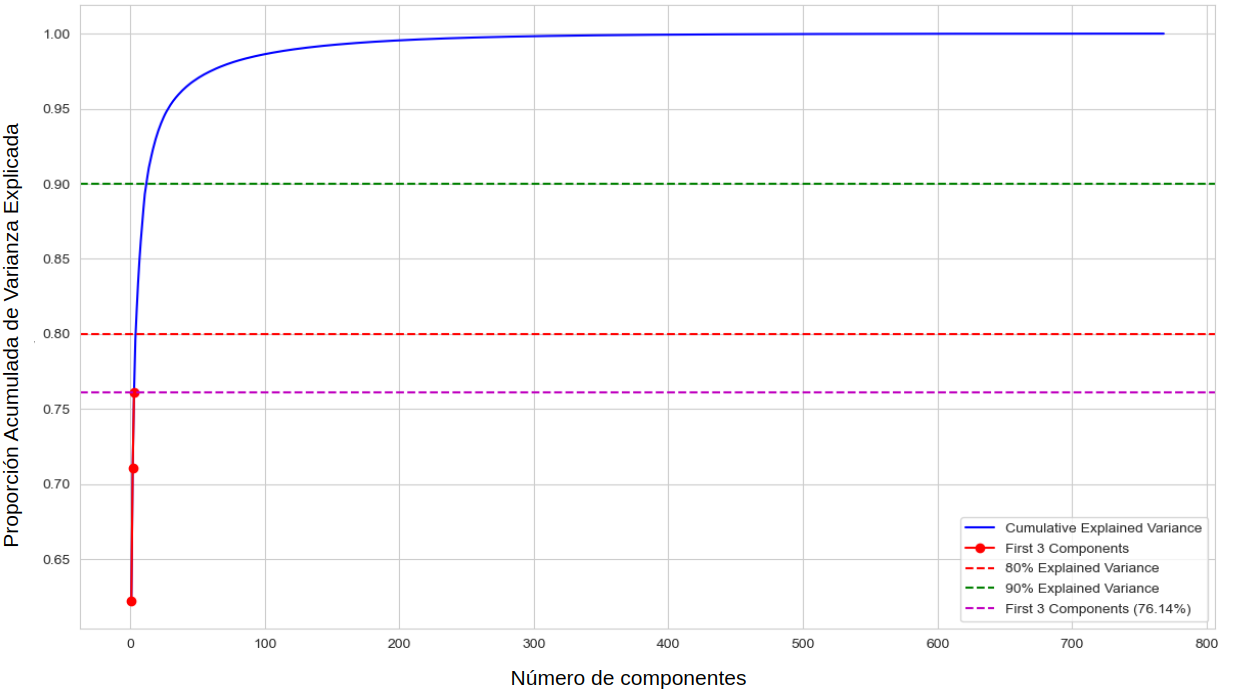
\includegraphics[width=0.6\textwidth]{imagenes/varianza-explicada.png}
    \caption{Varianza explicada en relación a la cantidad de componentes .}
\end{figure}

Esta varianza explicada se la comparó con la de trabajos similares, como el de \emph{user2-code2vec: Embeddings for Profiling Students Based on Distributional Representations of Source Code} \cite{user2code} en el que proponen una metodología para perfilar a estudiantes individuales de ciencias de la computación según su diseño de programación, utilizando \emph{embeddings}. Azcona et al. mencionan que, hablando de los embeddings con los que estaban trabajando, \emph{Los vectores se transforman a 2 dimensiones utilizando PCA. La varianza retenida es muy baja (entre 2\% y 6\%)}. Cabe destacar igualmente que, si bien a raíz de lo anterior no se esperaba una varianza explicada muy alta, en el trabajo de Azcona et al. el tamaño de los vectores generados es casi veinte veces mayor que el de los generados por \emph{CodeBERT}.

\subsection{Extracción de información adicional}\label{subsec:extraccion}

Sabemos que \emph{CodeBERT} captura la conexión semántica entre el lenguaje natural y el lenguaje de programación~\cite{codeBert}. En un análisis preliminar se investigó qué factores podían llegar a generar \emph{embeddings} diferentes para códigos semánticamente similares o idénticos. Con esto se esperaba encontrar características en el código sobre las cuales hacer foco para mejorar las futuras predicciones, de ser necesario. 

Para ello, se tomó una producción de código de un alumno al azar del ejercicio de la primer unidad, \emph{tiene\_a}, el cual debeía retornar $True$ de contener el \emph{string} a analizar la letra \emph{a}. A este se le hicieron pequeñas modificaciones, como, por ejemplo:
\begin{enumerate}
    \item Modificación del nombre de las variables.
    \item Cambio del $while$ en el recorrido por un $for$.
    \item Inversión en el recorrido de la secuencia (en vez de principio a fin de fin a principio).
    \item Agregado de prints.
    \item Simplificación del código.
\end{enumerate}

Entre otros. Se obtuvo lo siguiente:

\begin{figure}[H]
    \centering
    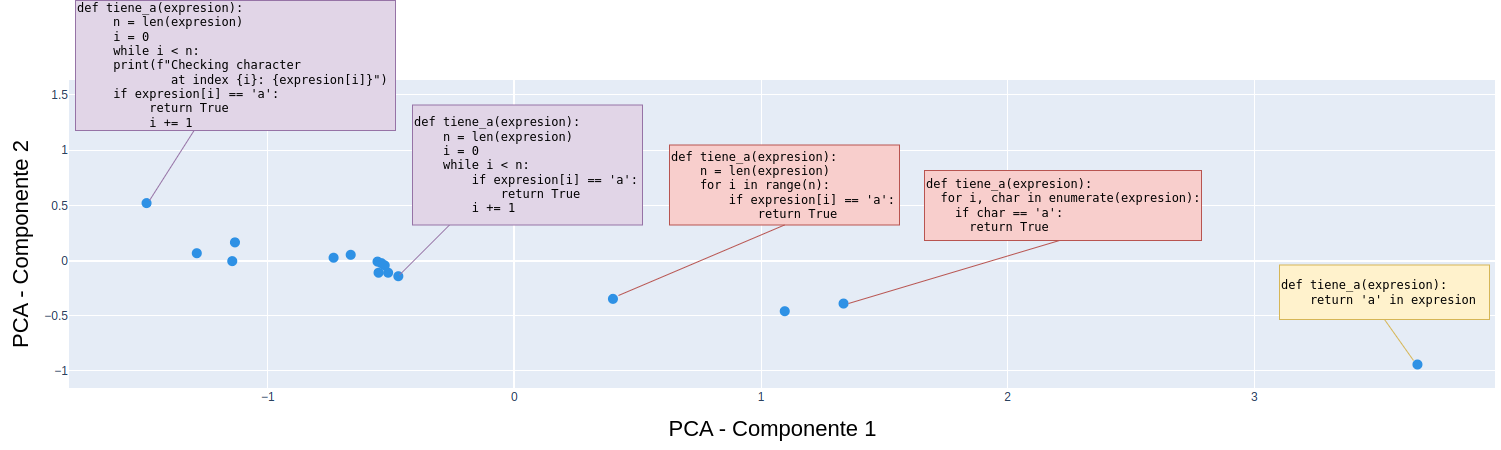
\includegraphics[width=\textwidth]{imagenes/codigo-similar.png}
    \caption{Representación de los dos primeros componentes de diferentes variantes del ejercicio \emph{tiene\_a}.}
\end{figure}

Como era de esperarse, se observó que variantes muy similares del código (como, por ejemplo las propuestas por los ítems 1) y 3)) no se distanciaban mucho las unas de las otras. En la figura anterior se puede observar también una clara tendencia en cuanto a la longitud del código y su representación en el plano. Además, diferencias cómo el uso de $for$ (los tres puntos comprendidos entre las dos cajas rojas) y el $while$ (aquellos comprendidos entre las cajas violetas) o la ausencia de ambos, tuvieron también un impacto significativo en los \emph{embeddings} y su representación en el plano de dos dimensiones.

A partir de lo anterior y, como se refleja en la Figura \ref{diagrama-base}, se tuvieron en cuenta para caracterizar cada código información como su uso de $for$, $while$, la cantidad de $if$ y la cantidad de líneas dentro de otras que surgieron a raíz de repetir el análisis anterior con otros ejercicios.

\subsection{Kmeans}

El algoritmo \emph{K-means} es una técnica de aprendizaje no supervisado ampliamente utilizada para resolver problemas de agrupamiento. Funciona dividiendo un conjunto de datos en \emph{k} \emph{clusters} ó grupos distintos. 

Primero, el algoritmo selecciona aleatoriamente \emph{k} centroides iniciales, que representan los centros de los \emph{clusters}. Luego, asigna cada punto de datos al \emph{cluster} cuyo centro esté más cercano, basado en la distancia euclidiana. Una vez asignados todos los puntos, se recalculan los centroides como la media de los puntos en cada \emph{cluster}. Este proceso de asignación y actualización de centroides se repite iterativamente hasta que las posiciones de los centroides ya no cambien significativamente, indicando que el algoritmo convergió. \cite{kmeans}

Sin embargo, el algoritmo \emph{K-means} presenta muchos desafíos que afectan negativamente su rendimiento. En primer lugar, en el proceso de inicialización del algoritmo uno debe especificar \emph{a priori} el número de grupos en un conjunto de datos dado (el número \emph{k}), mientras que los centros de los grupos iniciales se seleccionan aleatoriamente. Además, el rendimiento del algoritmo es susceptible a la selección de este grupo inicial y, para conjuntos de datos grandes, determinar el número óptimo de grupos con el que comenzar se vuelve desafiante. Más aún, la selección aleatoria de los centros de los grupos iniciales a veces resulta en una convergencia local mínima debido a que se trata de un algoritmo \emph{greedy}. \cite{kmeans-limitaciones}.

Este algoritmo y otras variantes que serán mencionadas a continuación se utilizará para intentar discriminar entre qué alumnos finalizarán o no el curso. 

\subsubsection{Elección del número de clusters} \textbf{ } 


Teniendo en cuenta las limitaciones mencionadas anteriormente, se eligió el \textbf{método del codo} para elegir el número \emph{k} a la hora de realizar los \emph{clusterings} que detallaremos en secciones posteriores. Esta es una técnica visual que ayuda a optimizar el número de grupos a utilizar en \emph{K-means}. Su objetivo principal es ayudar a tomar una decisión informada sobre cuántos \emph{clusters} elegir.

El método funciona de la siguiente manera:
\begin{enumerate}
    \item Se ejecuta el algoritmo de \emph{clustering} varias veces con diferentes números de \emph{clusters}.
    \item Para cada \emph{k}, se calcula la suma de los errores cuadráticos dentro del \emph{cluster} (\emph{WCSS}, por sus siglas en inglés).
    \item Se grafica el \emph{WCSS} en función del número de clústeres.
    \item Se busca un ``codo'' en el gráfico, que es un punto donde la disminución del \emph{WCSS} comienza a nivelarse.
\end{enumerate}

El ``codo'' en el gráfico representa el punto donde agregar más clústeres no mejora significativamente la calidad del agrupamiento. Este punto se considera el número óptimo de clústeres. Para ello, se calcula el error cuadrático total (SSE, por sus siglas en inglés) para diferentes cantidades de \emph{clusters}. El SSE mide la suma de las distancias cuadradas de cada punto al centroide más cercano, y se grafica frente al número de \emph{clusters}. En el gráfico, inicialmente el SSE disminuye rápidamente con el aumento de \emph{clusters}, pero en cierto punto la disminución se ralentiza, formando un ``codo'' en la curva. Este punto de inflexión indica el número óptimo de \emph{clusters}.

El método es beneficioso porque optimiza la elección del número de clusters eliminando la necesidad de depender de suposiciones previas \cite{metodo-codo}.


\subsubsection{Fuzzy-c-means} \textbf{ }

El algoritmo \emph{Fuzzy-c-means} es una técnica de agrupamiento que optimiza una función objetivo. Esta función minimiza la distancia entre los puntos de datos y los centros de los \emph{clusters}, ponderada por los valores de pertenencia difusa. El algoritmo itera entre actualizar los valores de pertenencia y los centros de los \emph{clusters} hasta alcanzar la convergencia. 

Entre las ventajas del \emph{Fuzzy-c-means} se encuentra su capacidad para permitir la pertenencia parcial a múltiples \emph{clusters}, lo que lo hace más flexible que los métodos de agrupamiento tradicionales. Además, maneja bien \emph{clusters} de formas no esféricas y es más robusto ante \emph{outliers} en comparación con el algoritmo \emph{k-means} que mencionamos anteriormente.

Sin embargo, este algoritmo, al igual que \emph{K-means},  \emph{Fuzzy-c-means} también requiere que se especifique el número de grupos \emph{a priori}. En consecuencia, también es sensible a la inicialización, lo que puede afectar los resultados finales. Además, tiene un mayor costo computacional en comparación con \emph{K-means}.

Chan et al. en ``Clustering of clusters'' introducen una variante llamada \emph{Recursive Fuzzy-2-Mean} (RF2M), que extiende el \emph{Fuzzy-c-means} para agrupar \emph{clusters} existentes. Esta variante introduce una tercera clase para los puntos que no encajan bien en ninguno de los dos \emph{clusters} principales, añadiendo así más flexibilidad al método original \cite{fuzzy-k-means}.


\subsubsection{Evaluación} \textbf{ }

\textbf{Adjusted Rand Index}

El \textit{Adjusted Rand Index} (ARI) es una métrica utilizada para determinar la similitud entre dos resultados de agrupamiento (\emph{clustering}). La fórmula del ARI es:

\begin{equation}
\text{ARI} = \frac{\text{RI} - \text{esperadoRI}}{\max \text{RI} - \text{esperadoRI}}
\end{equation}

donde \textit{RI} representa el índice de Rand, que calcula la similitud entre dos resultados de \emph{clustering} al considerar todos los puntos identificados dentro del mismo clúster. El valor del ARI es igual a 0 cuando los puntos se asignan aleatoriamente a los clústeres y es igual a 1 cuando los dos resultados de \emph{clustering} son idénticos. Esta métrica es útil para evaluar si los resultados de agrupamientos reducidos dimensionalmente son similares entre sí \cite{ari}.

\textbf{Normalized Mutual Information}

El \textbf{NMI} (Normalized Mutual Information) es una métrica utilizada para evaluar la calidad de las particiones en la detección de comunidades en redes. Esta métrica mide la similitud entre la partición obtenida por un algoritmo de detección de comunidades y una partición de referencia (también llamada \emph{ground truth}). El NMI está normalizado para variar entre 0 y 1, donde 1 indica una coincidencia perfecta entre las particiones y 0 indica que no hay relación alguna entre ellas.

La fórmula para calcular el NMI es la siguiente:

\[
\text{NMI} = \frac{2 \cdot I(X; Y)}{H(X) + H(Y)}
\]

donde \( I(X; Y) \) representa la información mutua entre las particiones \(X\) y \(Y\), y \( H(X) \) y \( H(Y) \) son las entropías de \(X\) y \(Y\), respectivamente. Esta métrica es utilizada para comparar las divisiones obtenidas por diferentes métodos y verificar qué tan similares son a la partición de referencia, proporcionando una medida cuantitativa de la precisión en la detección de comunidades \cite{nmi}.

\textbf{Similitud de Jaccard}

El índice de similitud de Jaccard es una medida utilizada para calcular la similitud entre dos conjuntos. Dados dos conjuntos \( A \) y \( B \), el índice de Jaccard se define como el tamaño de la intersección dividido por el tamaño de la unión de los conjuntos. Formalmente, se expresa como:

\[
J(A, B) = \frac{|A \cap B|}{|A \cup B|}
\]

donde:
\begin{itemize}
    \item \( |A \cap B| \) representa el número de elementos que son comunes a ambos conjuntos \( A \) y \( B \).
    \item \( |A \cup B| \) representa el número total de elementos únicos presentes en al menos uno de los conjuntos.
\end{itemize}

Una forma alternativa de expresar esta fórmula es:

\[
J(A, B) = \frac{m_{11}}{m_{10} + m_{01} + m_{11}}
\]

donde:
\begin{itemize}
    \item \( m_{11} \) es el número de elementos presentes en ambos conjuntos.
    \item \( m_{10} \) es el número de elementos presentes en \( A \) pero no en \( B \).
    \item \( m_{01} \) es el número de elementos presentes en \( B \) pero no en \( A \).
\end{itemize}

El índice de Jaccard es útil para medir la similitud entre conjuntos en diversas aplicaciones, como la minería de datos y la comparación de características en grandes espacios de atributos. La métrica ignora las no-ocurrencias compartidas entre los conjuntos, ya que estas no proporcionan información relevante sobre su similitud \cite{jaccard}.


\subsection{Consideraciones sobre múltiples entregas}

Finalmente, mencionamos que los estudiantes tenían la posibilidad de entregar un ejercicio las veces que quisieran. Para simplificar el análisis, si bien se cargaron a la base todas las entregas de las unidades mencionadas, se consideraron únicamente las entregas finales de cada alumno. Este filtrado se realizó rápidamente ya que contábamos con el \emph{Timestamp} de cada archivo.


\chapter{Resultados y discusión}
\section{Ejercicio a ejercicio}

En una primera instancia, se evaluó ejercicio a ejercicio entregable la distancia euclidiana entre los puntos generados después de realizar la mencionada reducción de la dimensionalidad para los alumnos en cada una de las 31 funciones. Con esto se esperaba ver grupos bien definidos y una correlación en cada instancia de evaluación entre ellos y los grupos de interés (esto es, estudiantes que terminaron \emph{vs} los que no). 

Para ello, se graficaron varios \emph{heatmaps} esperando ver en ellos distintos grupos de alumnos. 

Se observó que, en ejercicios que podrían considerarse más sencillos como, por ejemplo, el ejercicio \emph{tirar} de la unidad 5 que consistia en obtener el resultado de tirar un dado equilibrado de seis caras \emph{n} veces, o \emph{crear\_album} de la misma unidad que consistía en crear un ``álbum'' (un vector de ceros) de \emph{n} figuritas, habían grupos claramente definidos, como se observa en las siguientes figuras:
\begin{figure}[H]
    \centering
    \begin{subfigure}{0.45\textwidth}
        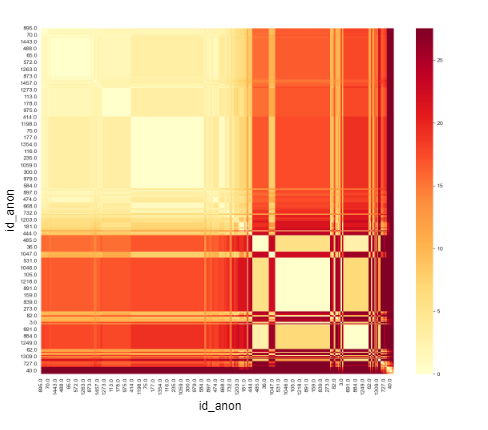
\includegraphics[width=\linewidth]{imagenes/heatmap-1-crear album.png}
        \caption{Heatmap del ejercicio \emph{crear\_album}}
        \label{fig:figura1}
    \end{subfigure}
    \hfill
    \begin{subfigure}{0.45\textwidth}
        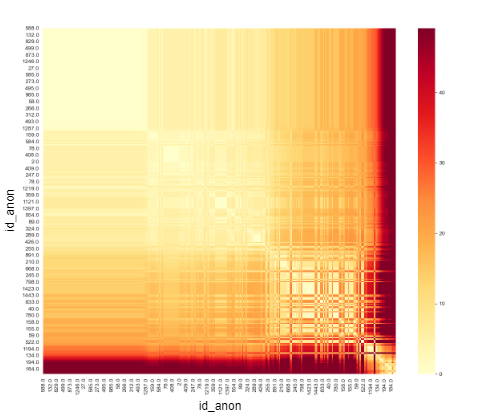
\includegraphics[width=\linewidth]{imagenes/heatmap-1-tirar.png}
        \caption{Heatmap del ejercicio \emph{tirar}}
        \label{fig:figura2}
    \end{subfigure}
    \caption{Ejemplos de ejercicios con grupos marcados, analizando las distancias entre las entregas de cada alumno con cada alumno}
    \label{fig:figuras_juntas}
\end{figure}

En otros ejemplos, en los cuales los ejercicios podían llegar a presentar una mayor dificultad o ambigüedad para los alumnos, los grupos no fueron tan claros. Este es el caso, por ejemplo, de los ejercicios \emph{es\_generala} de la unidad cinco y \emph{propagar} de la unidad cuatro. Para la primera, el comportamiento esperado para la función era que retornara \emph{True} si y sólo si los cinco dados de la lista tirada eran iguales. Para el segundo mencionado, los estudiantes debían escribir una función que recibiera una lista de fósforos (0: nuevo, 1: encendido, -1: carbonizado) y devolviera la lista con el fuego propagado a los fósforos nuevos adyacentes:

\begin{figure}[H]
    \centering
    \begin{subfigure}{0.45\textwidth}
        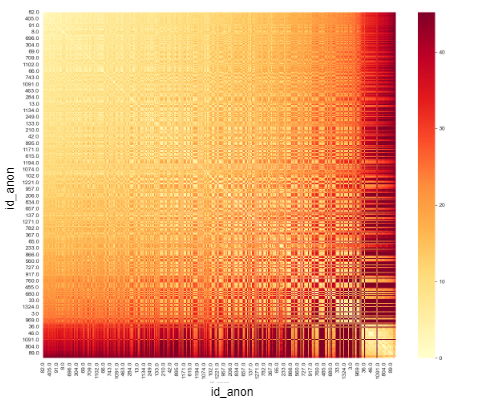
\includegraphics[width=\linewidth]{imagenes/heatmap-1-propagar.png}
        \caption{Heatmap del ejercicio \emph{propagar}}
        \label{fig:figura1}
    \end{subfigure}
    \hfill
    \begin{subfigure}{0.45\textwidth}
        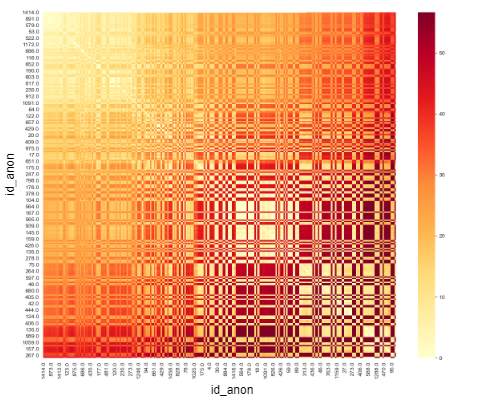
\includegraphics[width=\linewidth]{imagenes/heatmap-1-prob generala.png}
        \caption{Heatmap del ejercicio \emph{es\_generala}}
        \label{fig:figura2}
    \end{subfigure}
    \caption{Ejemplos de ejercicios con grupos no marcados, analizando las distancias entre las entregas de cada alumno con cada alumno}
    \label{fig:figuras_juntas}
\end{figure}

Cabe destacar que, a excepción de otros ejercicios típicamente introductorios en cursos como estos (como \emph{sumar}, \emph{máximo}, \emph{mínimo} dentro de otros), los gráficos como los que muestran las figuras anteriores fueron los predominantes, dando poca información. 

Se decidió entonces hacer foco en aquellos ejercicios en los que podían llegar a haber grupos mejor definidos. En un análisis posterior se exploró si estos grupos separaban de alguna manera a aquellos estudiantes que habían finalizado el curso de los que no. Para ello, se añadió la siguiente información a los gráficos anteriores:

\begin{figure}[H]
    \centering
    \begin{subfigure}{0.45\textwidth}
        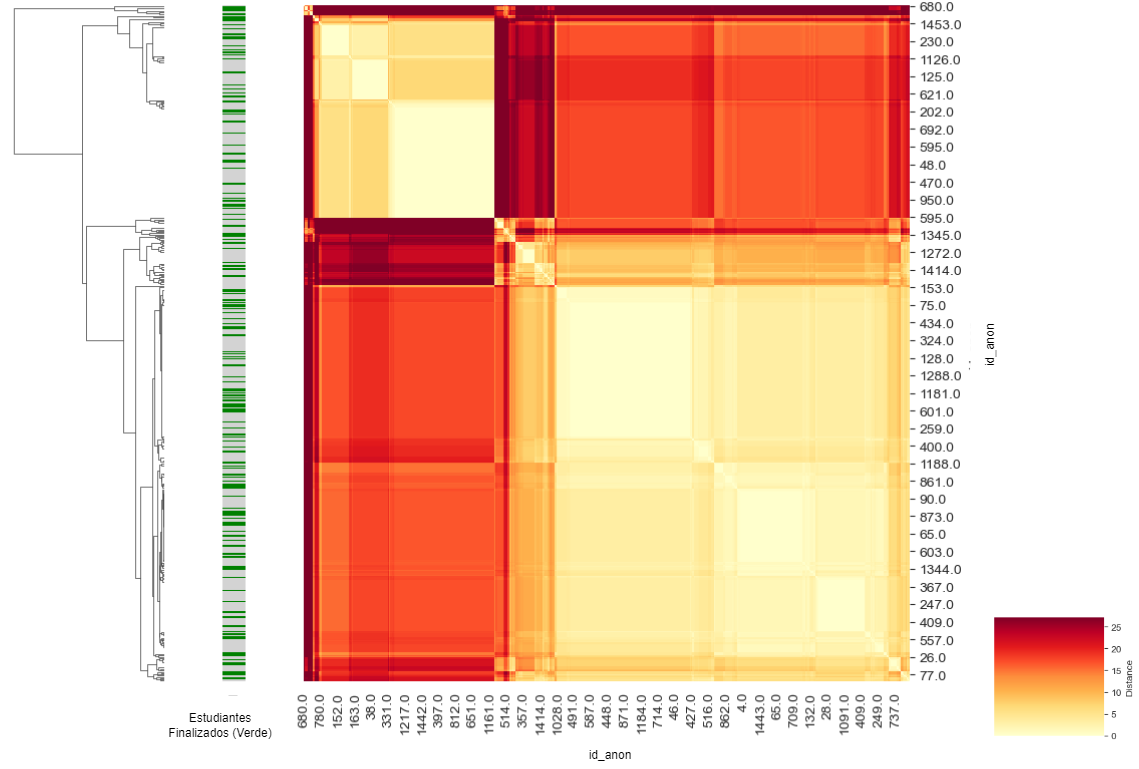
\includegraphics[width=\linewidth]{imagenes/heatmap-2-crear album.png}
        \caption{Heatmap del ejercicio \emph{crear\_album}}
        \label{fig:figura1}
    \end{subfigure}
    \hfill
    \begin{subfigure}{0.45\textwidth}
        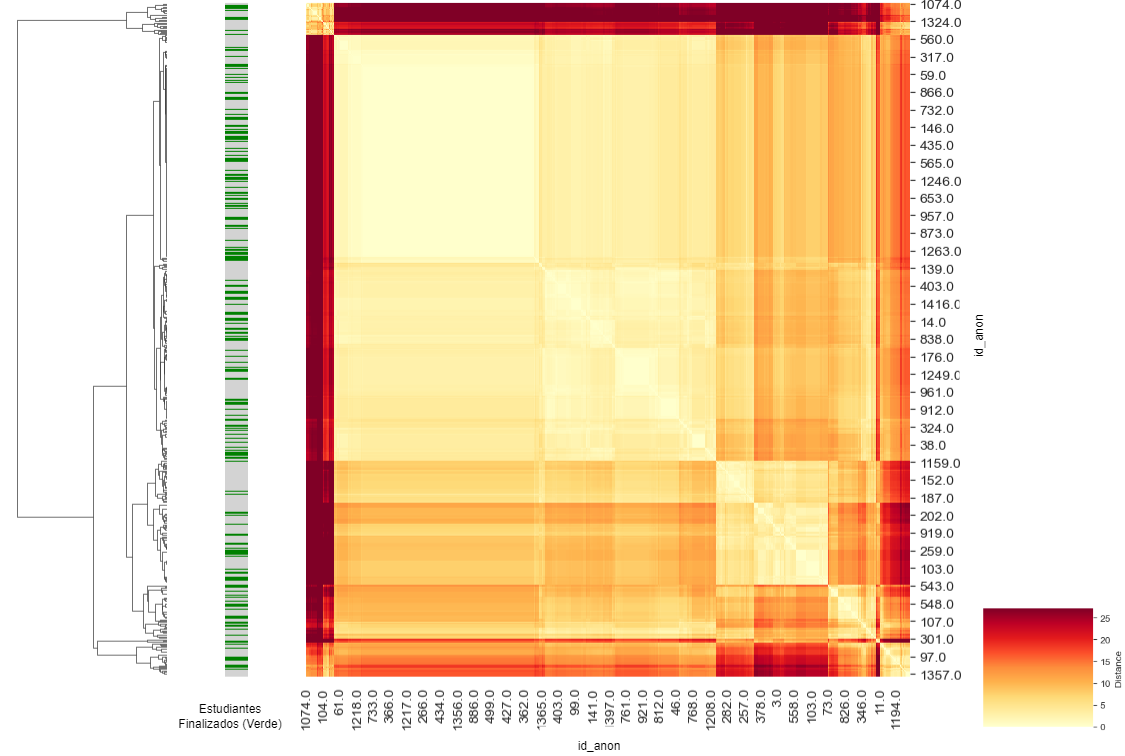
\includegraphics[width=\linewidth]{imagenes/heatmap-2-tirar.png}
        \caption{Heatmap del ejercicio \emph{tirar}}
        \label{fig:figura2}
    \end{subfigure}
    \caption{Ejemplos de ejercicios con grupos marcados, analizando las distancias entre las entregas de cada alumno con cada alumno con dendograma e indicador de qué estudiante finalizó el curso y cuál no.}
    \label{fig:figuras_juntas}
\end{figure}


Se observó que con los grupos obtenidos no era posible distinguir entre los dos grupos deseados analizando los ejercicios de manera individual. Esto se ve evidenciado en que los alumnos que abandonaron el curso se encuentran entremezclados con los que sí lo hicieron. Esta tendencia (o falta de ella) se vio en todos los \emph{heatmaps} que se realizaron. 


En un intento adicional por obtener información a partir de los ejercicios observados de manera atómica, se realizaron dos \emph{heatmaps} por ejercicio, ahora separando manualmente ambos grupos esperando ver sub-grupos diferenciados. Pero, como era de esperarse basándonos en el resultado anterior, la distribución de ambos grupos era similar, obteniéndose figuras muy similares a pesar de estar forzando esta distinción.

\section{Cluster a cluster}
Para esta sección, se analizaron varias métricas para evaluar el \emph{clustering} realizado. La evaluación rigurosa de los resultados del agrupamiento es fundamental por múltiples razones: permite validar la calidad de las agrupaciones obtenidas, asegura que los patrones descubiertos son significativos y no aleatorios, y facilita la comparación objetiva entre diferentes configuraciones del algoritmo. Además, dado que el \emph{clustering} es una técnica de aprendizaje no supervisado, estas métricas proporcionan una forma cuantitativa de verificar si los grupos identificados representan verdaderamente estructuras naturales en los datos.

\subsection{ARI y NMI}
Como se mencionó anteriormente, para cada ejercicio se realizó una \emph{clusterización} usando el método del codo. Para comparar las particiones generadas por cada ejercicio, se calcularon el ARI \cite{ari} y el NMI \cite{nmi} para todos los ejercicios analizados.

\begin{figure}[H]
    \centering
    \begin{subfigure}{0.45\textwidth}
        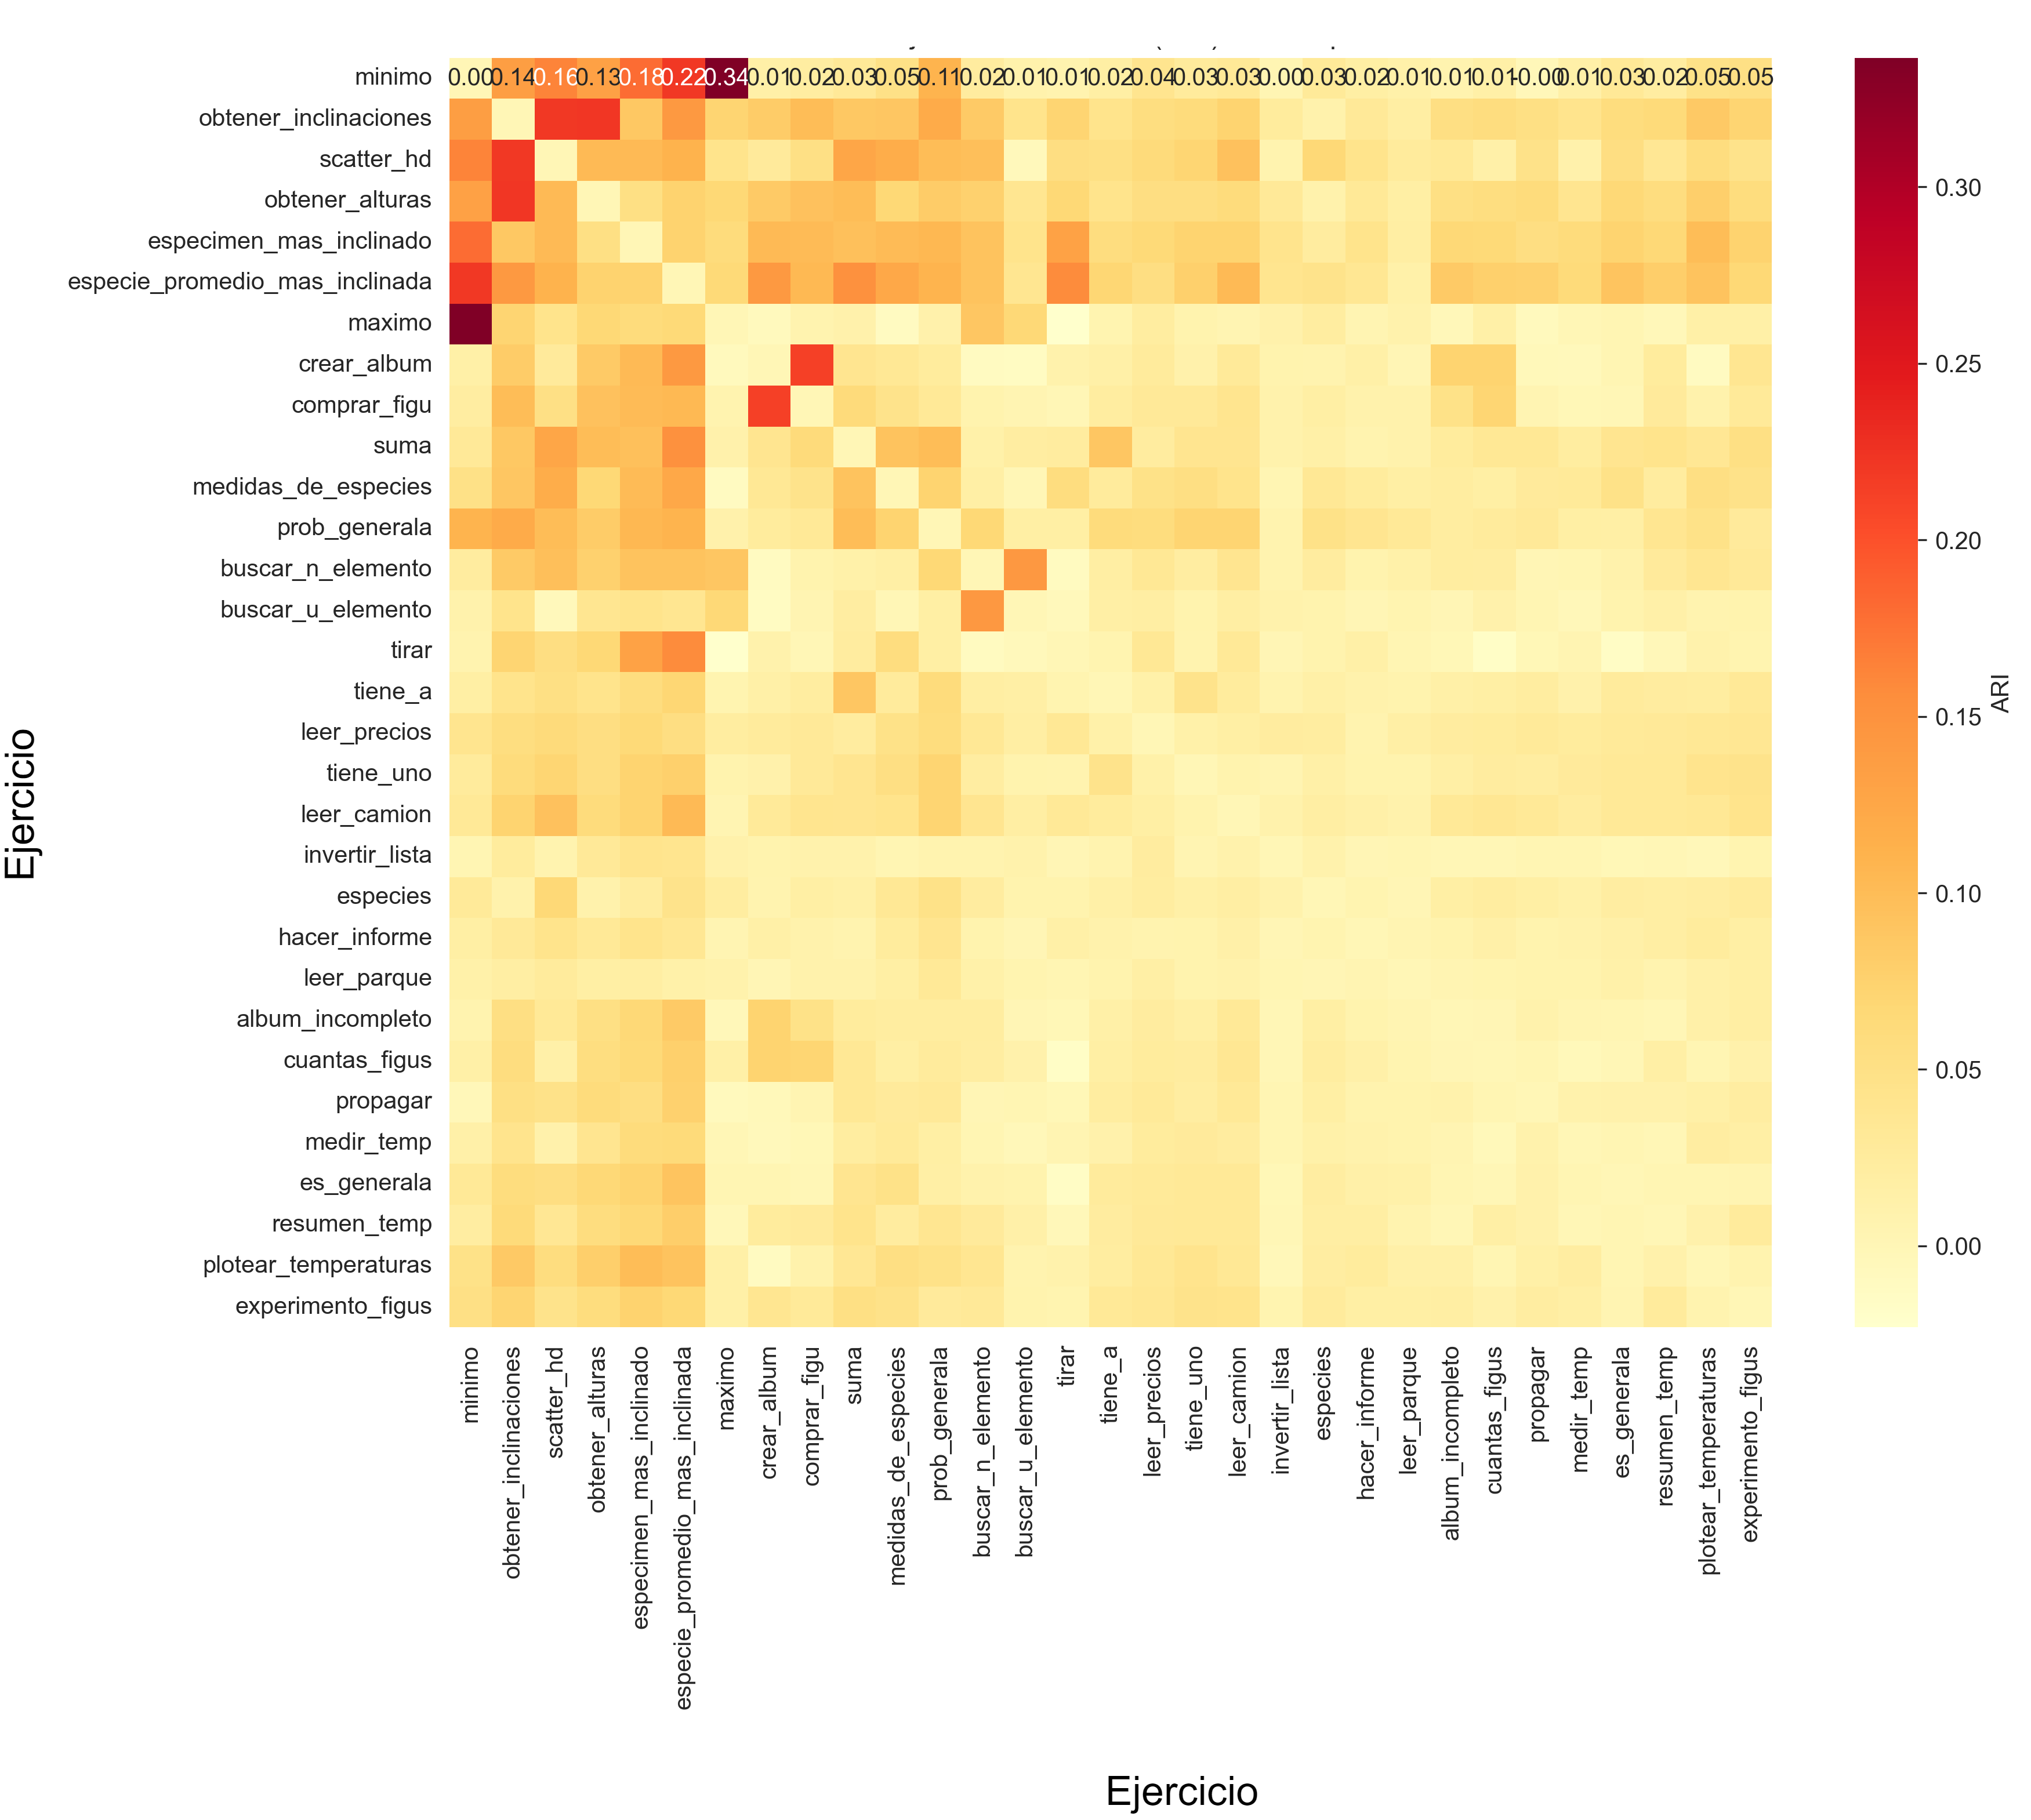
\includegraphics[width=\linewidth]{imagenes/ari.png}
        \caption{ARI}
        \label{fig:figura1}
    \end{subfigure}
    \hfill
    \begin{subfigure}{0.45\textwidth}
        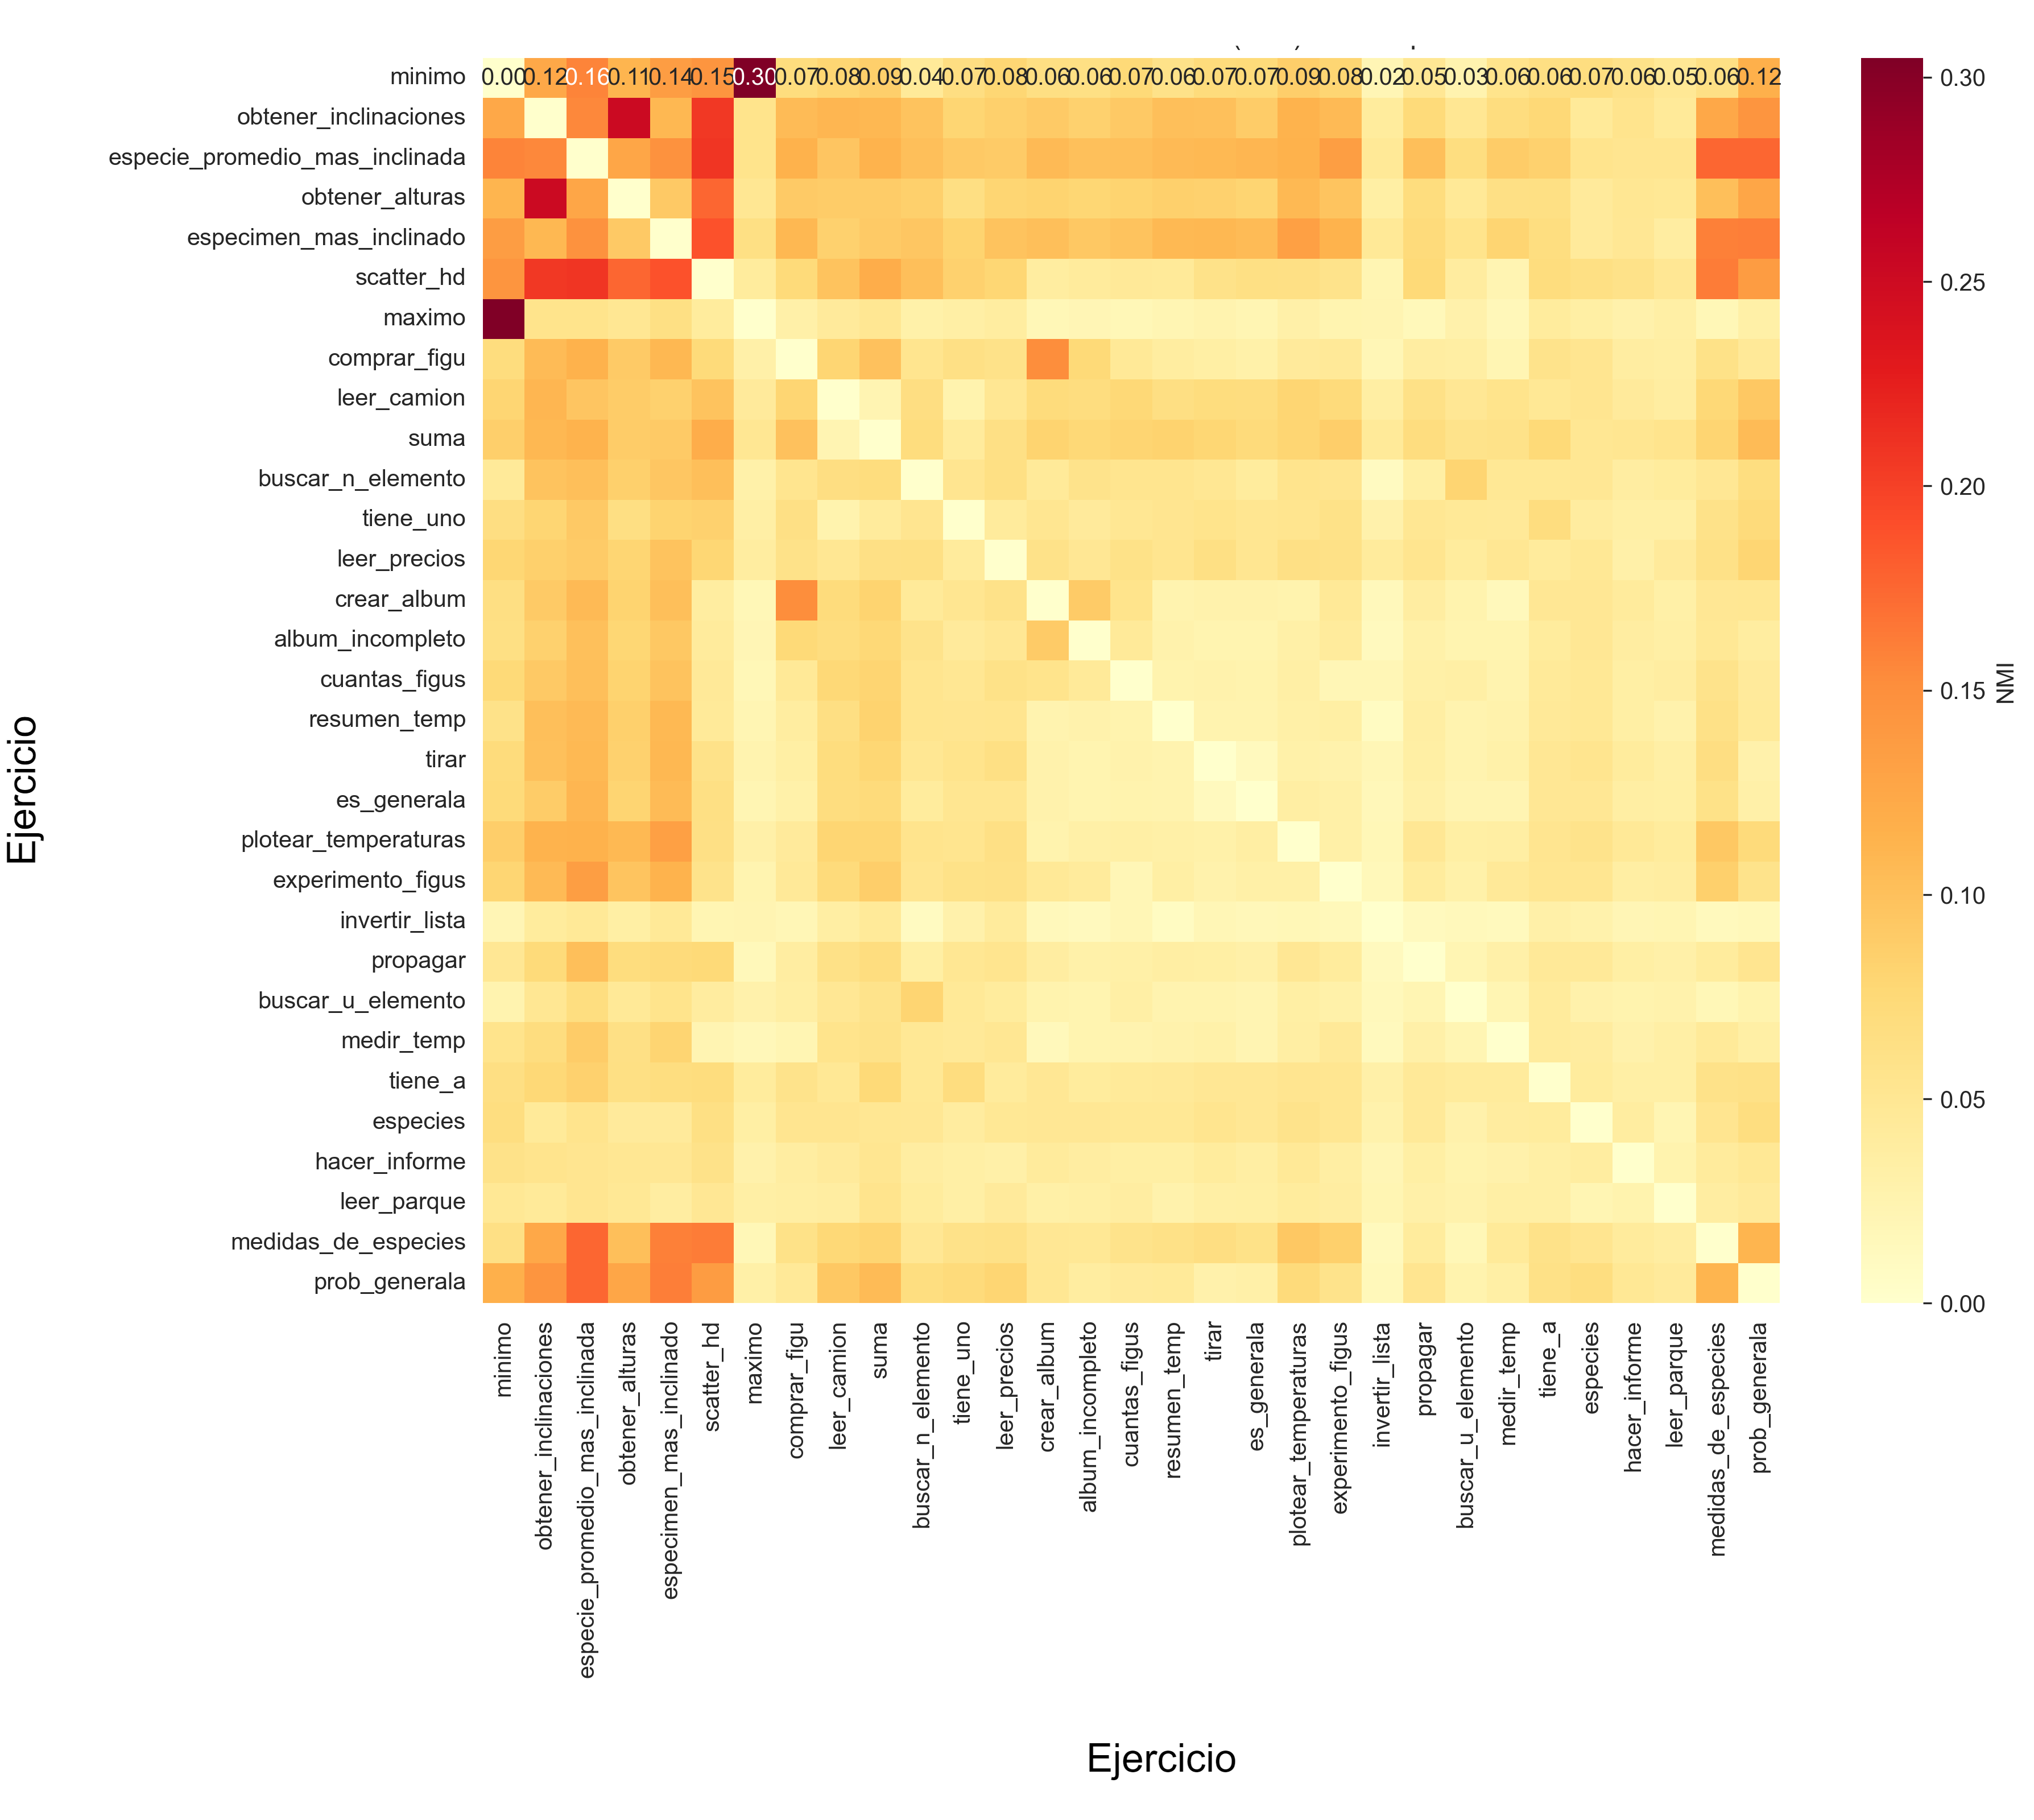
\includegraphics[width=\linewidth]{imagenes/nmi.png}
        \caption{NMI}
        \label{fig:figura2}
    \end{subfigure}
    \caption{\emph{Heatmaps} del ARI y NMI de todas las particiones generadas para cada ejercicio.}
    \label{fig:figuras_juntas}
\end{figure}

Los bajos valores de NMI sugieren que la información compartida entre las particiones detectadas y la referencia es mínima. Esto significa que las divisiones obtenidas por el algoritmo no están alineadas con las categorías del otro ejercicio con las que se las está comparando, lo que indica una posible falta de coherencia en la identificación de las comunidades o grupos en los datos.

Por otro lado, los bajos valores de ARI implican que la similitud entre las asignaciones de elementos a \emph{clusters} es baja en comparación con la asignación de referencia (o, como es este caso, a la partición generada para otro ejercicio).

\subsection{Índice de Jaccard}
Para esta evaluación se analizaron las particiones de manera individual. Esto es, obviando a qué ejercicio pertenecían, se calculó el Índice de Similitud de Jaccard \cite{jaccard} para cada uno de los más de cien \emph{clusters} generados a lo largo de los 31 entregables, obteniéndose lo siguiente:

\begin{figure}[H]
    \centering
    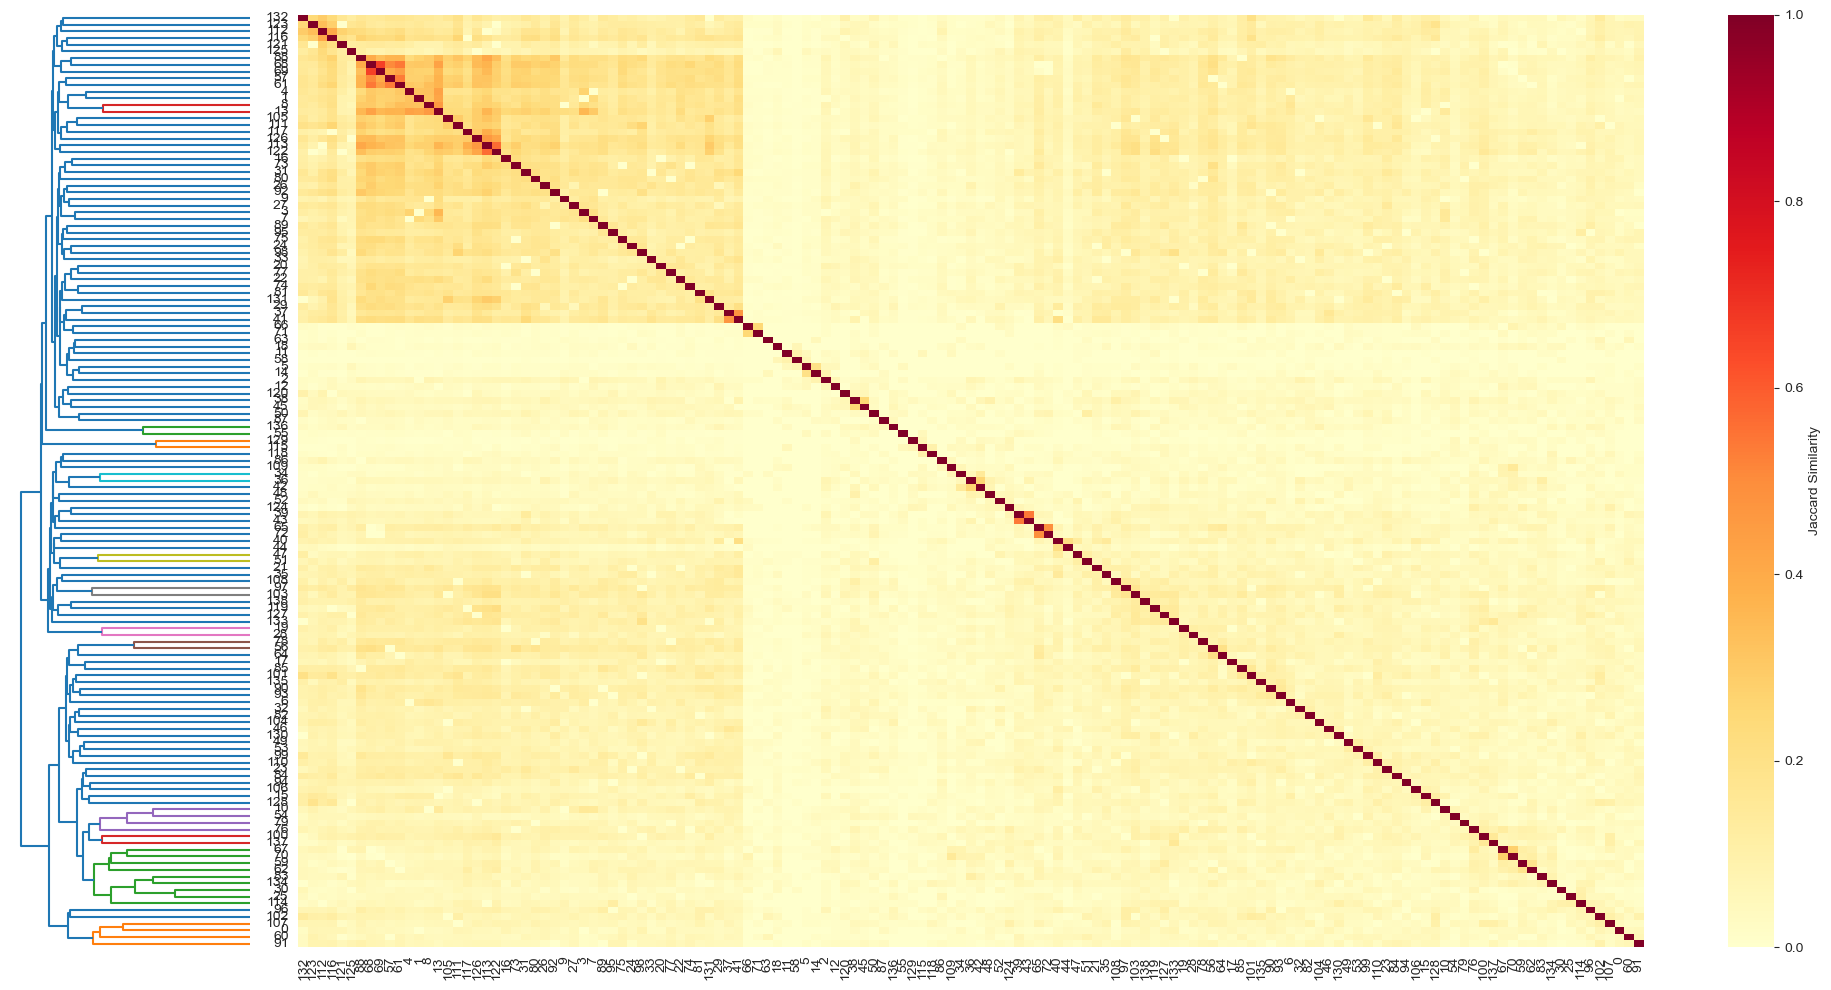
\includegraphics[width=0.7\textwidth]{imagenes/clusterxcluster.png}
    \caption{Índice de similitud de Jaccard entre todos los \emph{clusters} generados ejercicio a ejercicio.}
\end{figure}


Mencionan Loginova et al. sobre la caracterización de dos grupos de alumnos (\emph{low} y \emph{high achievers}) a través de \emph{embeddings} usando PCA y \emph{Kmeans} que \emph{...la mayoría de los clusters no son fácilmente interpretables, ya que contienen una mezcla de ambas clases, siguiendo aproximadamente la distribución de las etiquetas objetivo}\cite{loginova2021embedding}.


Cabe destacar que es razonable que entre \emph{clusters} de un mismo ejercicio, el Índice sea bajo. Esto puede ser un indicador de una buena separación entre los \emph{clusters}. Sin embargo, hubiera sido deseable que entre distintos ejercicios el Índice de Jaccard fuera alto, indicando que estas particiones se sostienen a lo largo del curso e, idealmente, un indicador de a qué grupo (ya sea deserción o finalización) del curso pertenecen los estudiantes. 

\section{Comparación por clusters en común}

Alineados con la idea de encontrar un patrón a lo largo de todos los ejercicios a analizar, se observaron ahora los \emph{clusters} en común para cada estudiante. Esto es, en vez de calcular \emph{cluster} a \emph{cluster} qué estudiantes tenían en común, se indagó sobre, estudiante a estudiante, qué \emph{clusters} tenían en común. 

\begin{figure}[H]

    \centering
    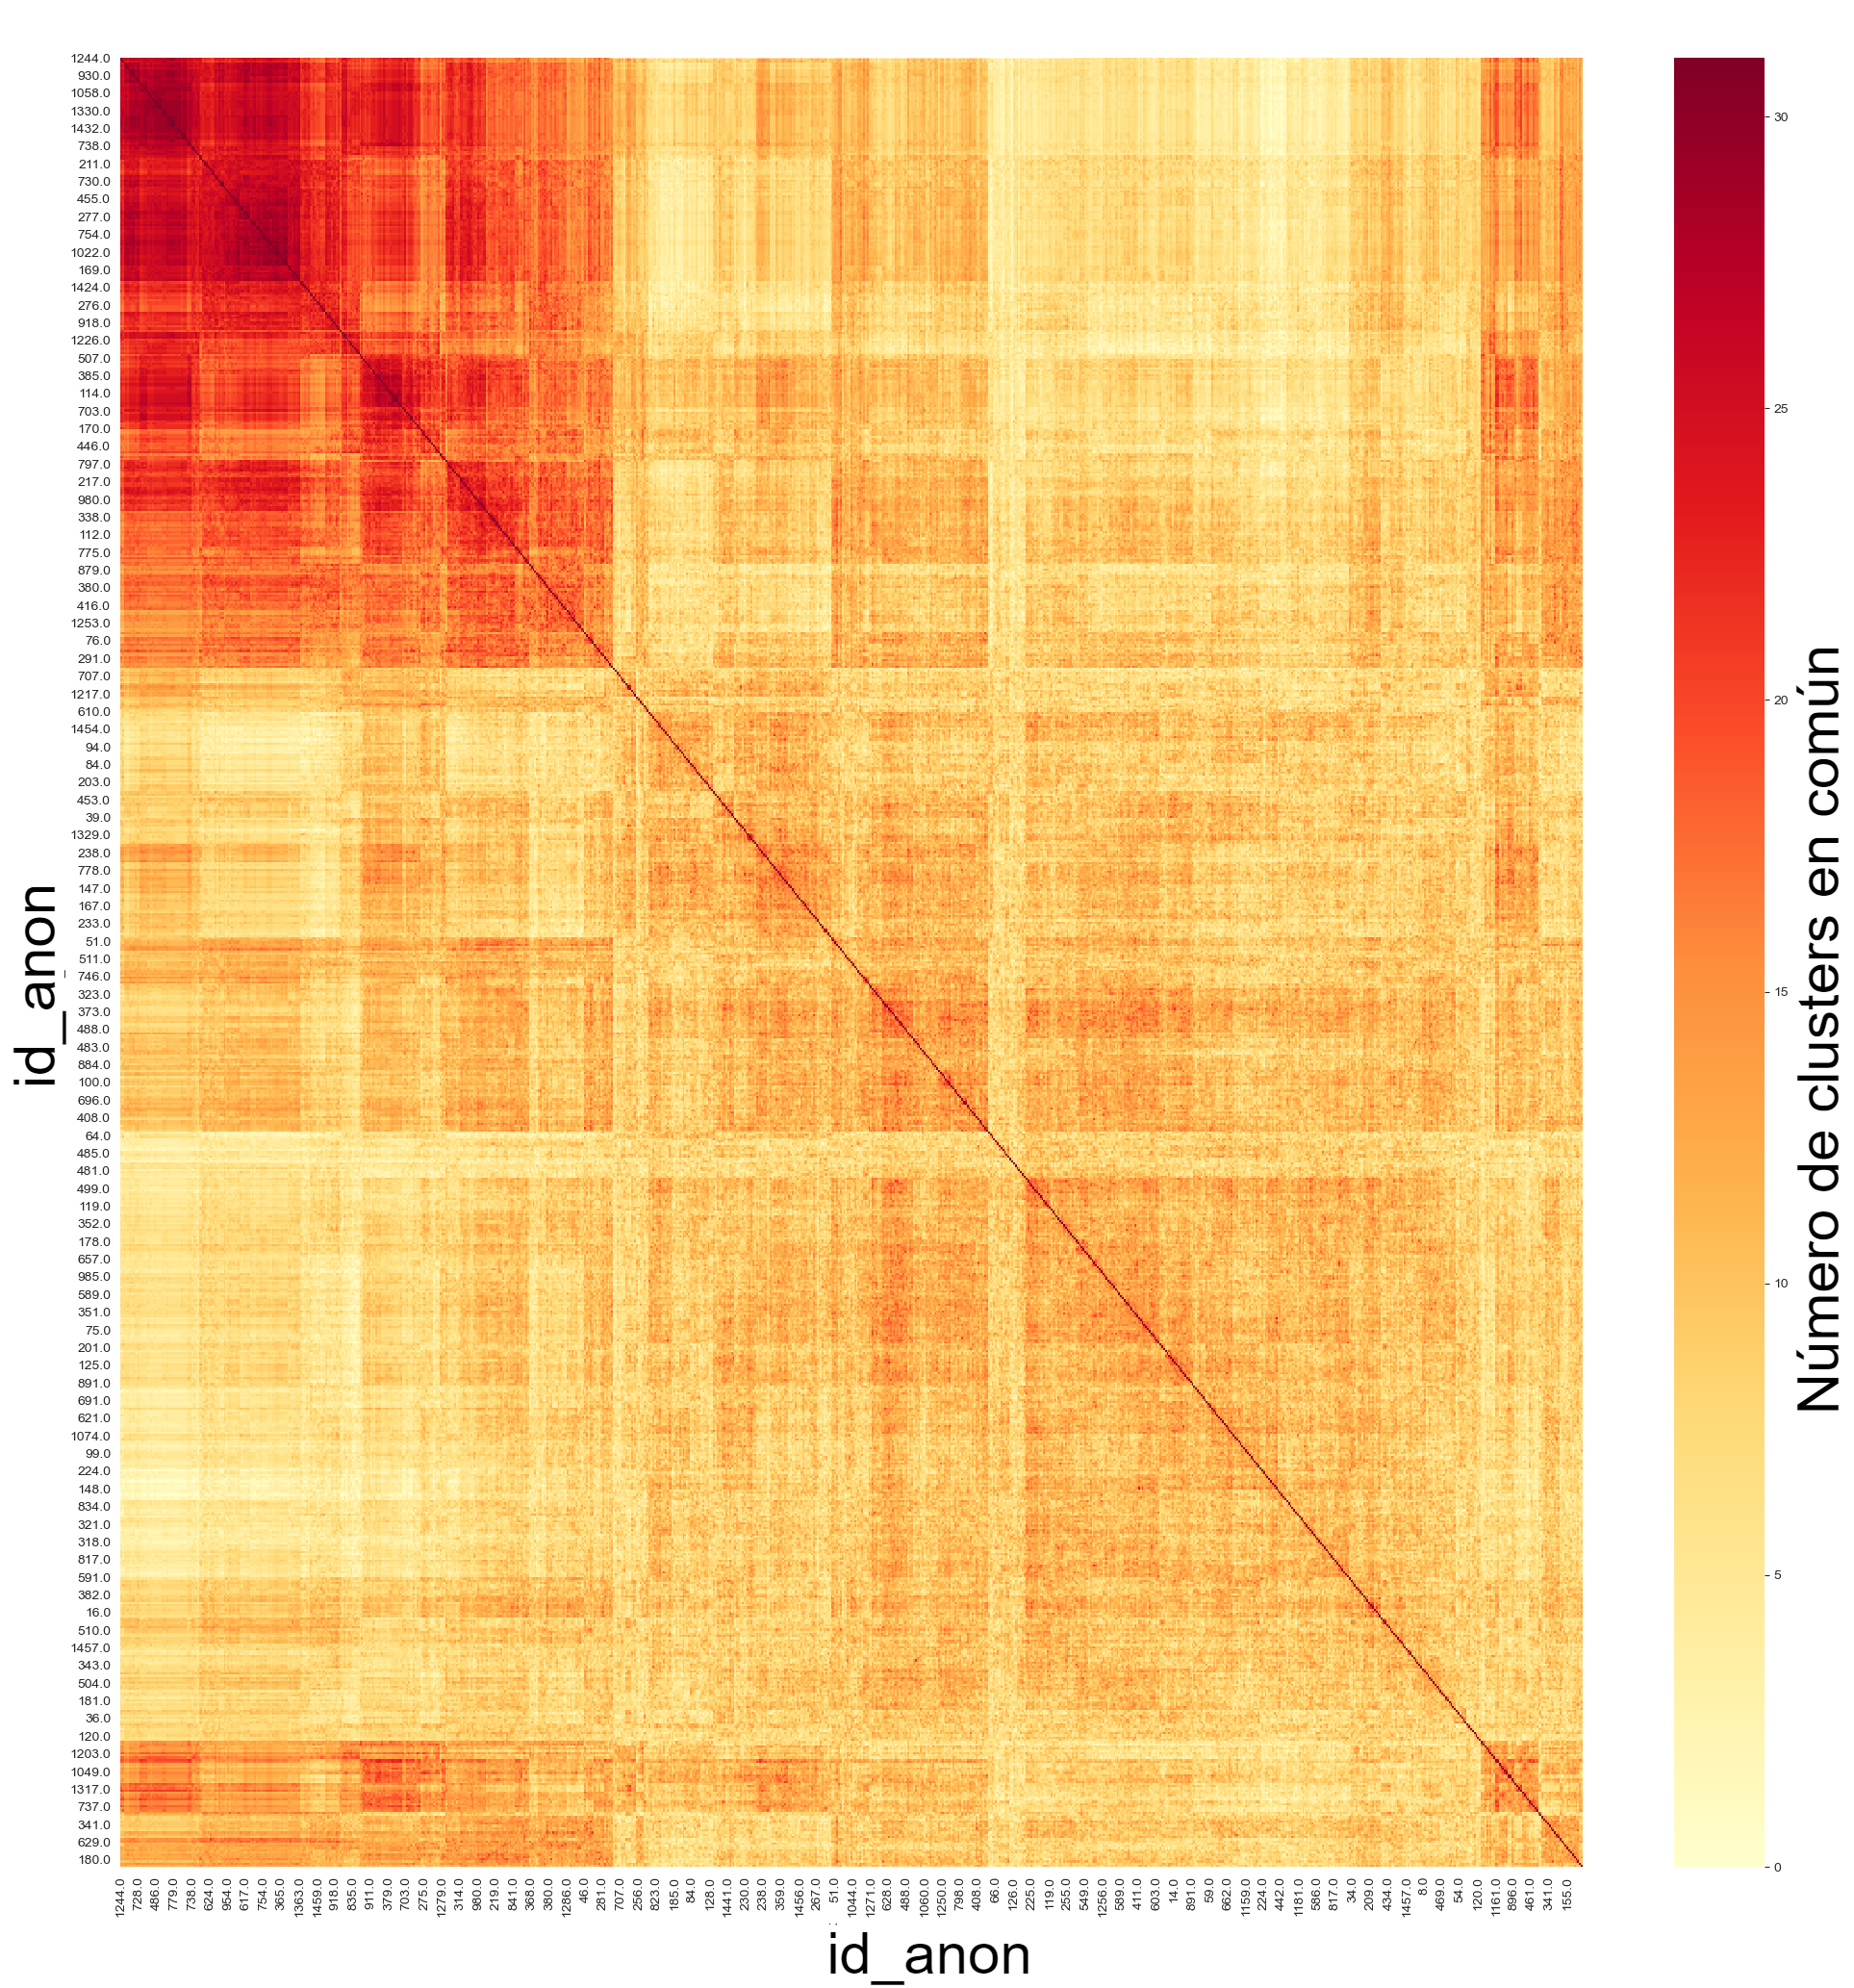
\includegraphics[width=0.5\textwidth]{imagenes/cluster.png}
    \caption{Cantidad de \emph{clusters} compartidos por estudiante.}
    \label{cluster}
\end{figure}

Se puede observar un grupo que comparte una gran cantidad de clusters en la esquina superior izquierda. Se buscó una manera de caracterizar este grupo, a partir de la matriz de \emph{clusters} compartidos generada para la realización del \emph{heatmap}. 


\subsection{Clique máximo}\textbf{ }
Usando la biblioteca Networkx \cite{networkx}, se buscó para diferentes cantidades de \emph{clusters} compartidos, el \emph{clique} más grande con el siguiente código:


\begin{algorithm}[H]
\caption{Encontrar el clique más grande con n clusters compartidos}
\begin{algorithmic}[1]
\Function{EncontrarCliqueMasGrande}{$n, \text{matriz\_de\_clusters\_compartidos}$}
    \State $G \gets \text{Crear grafo vacío}$
    \State $\text{id\_anons} \gets \text{índices de matriz\_de\_clusters\_compartidos}$
    \State Añadir nodos $\text{id\_anons}$ a $G$
    \For{cada par $(i, j)$ de nodos en $G$}
        \If{$\text{matriz\_de\_clusters\_compartidos}[i, j] \geq n$}
            \State Añadir arista $(i, j)$ a $G$
        \EndIf
    \EndFor
    \State $\text{cliques} \gets \text{Encontrar todos los cliques máximos en } G$
    \State $\text{clique\_mas\_grande} \gets \text{Clique más grande en cliques}$
    \State \Return $\text{clique\_mas\_grande}$
\EndFunction
\end{algorithmic}
\end{algorithm}

El código garantiza que todos los estudiantes en el \emph{clique} resultante comparten al menos \emph{n} \emph{clusters} entre sí debido a dos aspectos clave de su implementación. Primero, en la construcción del grafo, solo se crea una arista entre dos estudiantes si comparten \emph{n} o más \emph{clusters}. Esto significa que la existencia de una conexión en el grafo es equivalente a compartir al menos \emph{n} \emph{clusters}.

Segundo, el algoritmo busca el \emph{clique} más grande en este grafo. Por definición, un \emph{clique} es un subgrafo completamente conectado, lo que significa que todos los nodos en el \emph{clique} están conectados directamente entre sí. Como en este grafo cada conexión representa compartir al menos \emph{n} \emph{clusters}, todos los estudiantes en el \emph{clique} resultante necesariamente comparten al menos \emph{n} \emph{clusters} con todos los demás miembros del \emph{clique}. Así, la combinación de la construcción selectiva del grafo y la búsqueda de \emph{cliques} asegura la propiedad deseada.

En cuanto a la ejecución del algoritmo anterior, basados en la Figura \ref{cluster} se comenzó a iterar buscando el \emph{clique} más grande para cada \emph{n} comenzando desde el muy optimista número de más de veintitrés \emph{clusters} en común, descendientemente. Cabe destacar que estas corridas se hicieron por separado debido a los extensos tiempos de ejecución que estas llevaron y se eligió este número por representar ``más de la mitad del curso''. Más específico aún, se trata del número de la última entrega de la última unidad anterior al primer parcial (el ejercicio \emph{medidas\_especies}), momento para el cual sería deseable tener una noción de quiénes continuarán con el curso.   

Como es de esperarse, a medida que se decrementa dicho \emph{n}, la cantidad de alumnos en el \emph{clique} aumenta ya que se vuelve más laxa la condición para formar parte de él. Notamos sin embargo que, a medida que se reducía el \emph{n}, la proporción de alumnos que \emph{no habían terminado el curso} dentro del \emph{clique}, incrementaba.  Esta tendencia se observó hasta alcanzar los 13 \emph{clusters} en común, número a partir del cual la proporción comenzaba a disminuir nuevamente.

De este grupo de \emph{Clique-13} compuesto 222 estudiantes y representando un 27\% del alumnado, solo dos finalizaron el curso, siendo el restante 99\% del grupo más de la mitad (54\%) de los estudiantes que no terminaron el programa. 

Habiendo entonces caracterizado a más de la mitad, fue necesario entender qué entregas eran las que habían realizado de manera similar con el objeto de poder estimar en un futuro qué ejercicios podrían servir de guía para realizar estas estimaciones. 

A partir de este momento entonces se intentó caracterizar no a dos grupos si no a tres: aquellos que pertenecían a este grupo apodado \emph{Clique-13} que, en su vasta mayoría, no habían finalizado el curso, aquellos estudiantes que no pertenecían a los anteriores pero tampoco habían terminado la materia y, finalmente, los que continuaron con el programa hasta su finalización.

\subsection{Separación por grupos}\textbf{ }

Se analizó entonces qué ejercicios habían entregado cada grupo: 
\begin{figure}[H]
    \centering
    \begin{subfigure}[t]{0.3\textwidth}
        \centering
        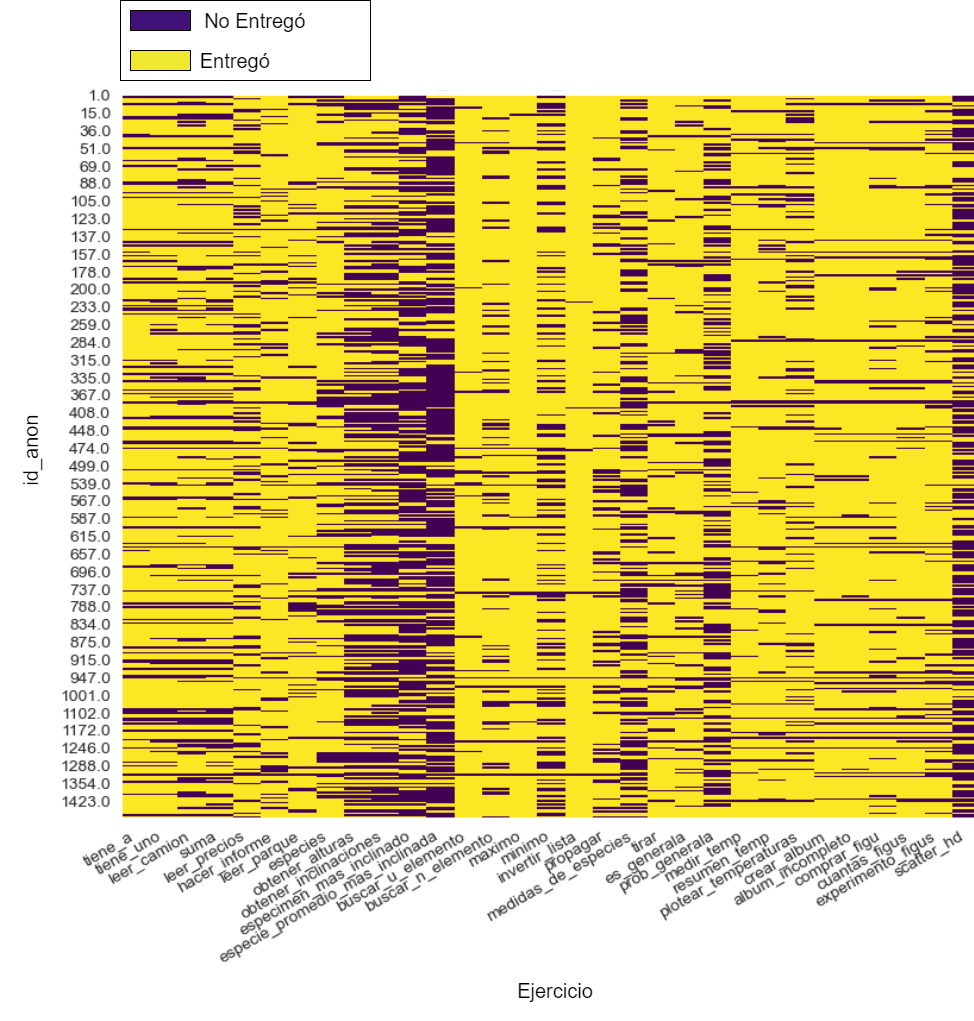
\includegraphics[width=\linewidth]{imagenes/entregas - finalizados.png}
        \caption{Alumnos que finalizaron el curso.}
        \label{fig:final}
    \end{subfigure}
    \hfill
    \begin{subfigure}[t]{0.3\textwidth}
        \centering
        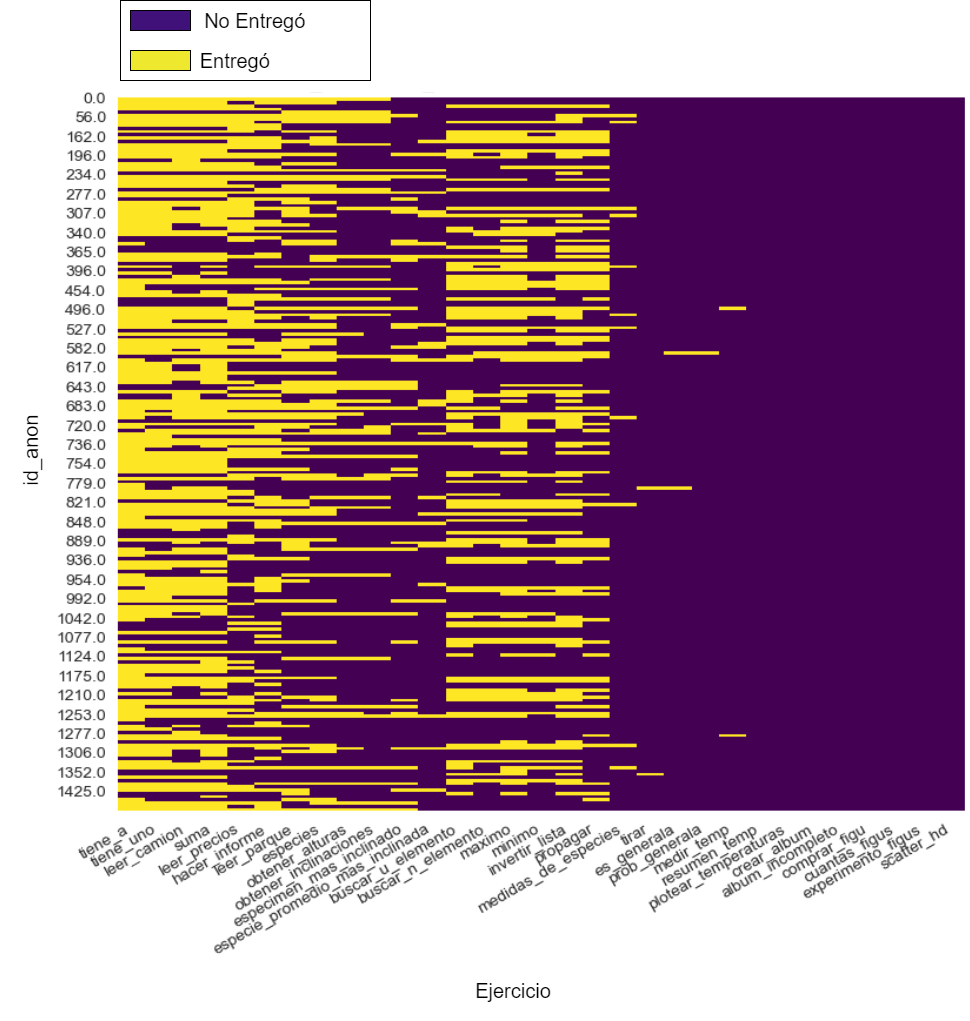
\includegraphics[width=\linewidth]{imagenes/entregas - clique13.png}
        \caption{Alumnos con más de 13 \emph{clusters} en común.}
        \label{fig:clique}
    \end{subfigure}
    \hfill
    \begin{subfigure}[t]{0.3\textwidth}
        \centering
        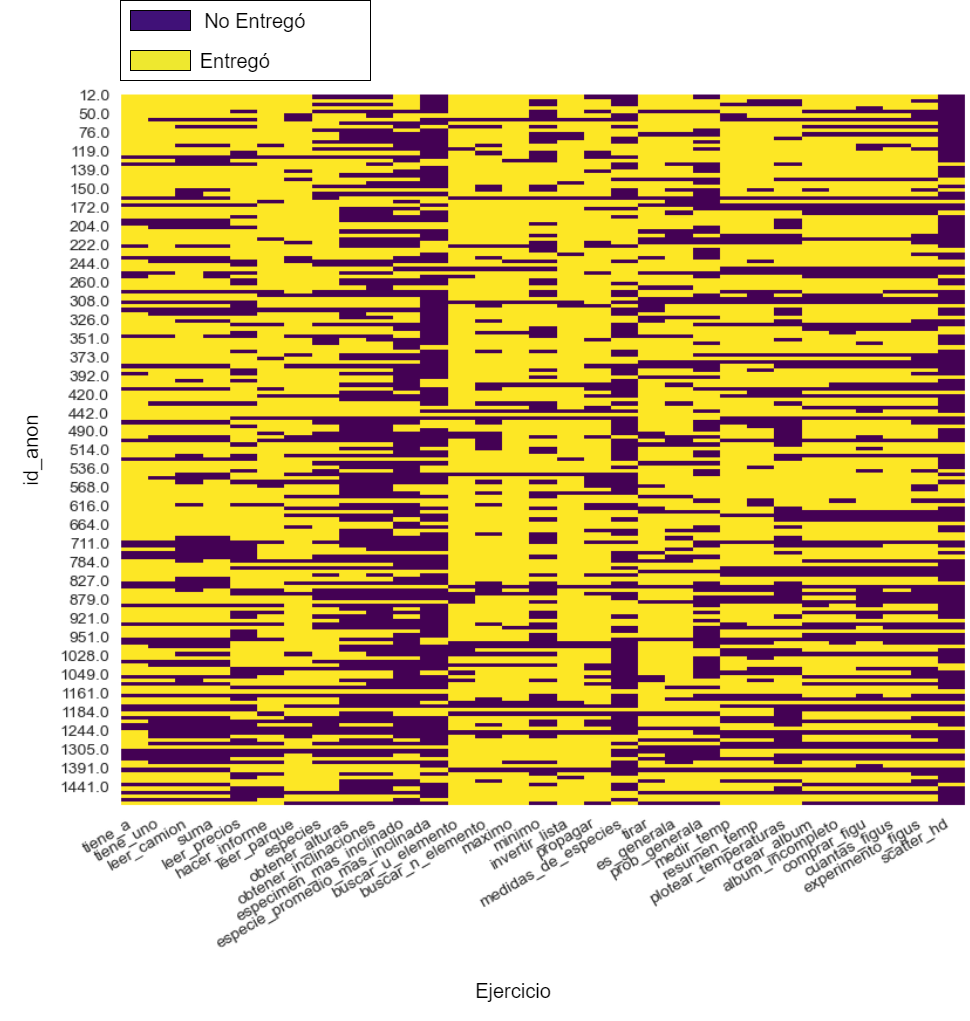
\includegraphics[width=\linewidth]{imagenes/entregas - no-clique13.png}
        \caption{Alumnos que no finalizaron el curso,\\que no pertenecen al grupo anterior.}
        \label{fig:noclique}
    \end{subfigure}
    \caption{Entregas por alumno según el ejercicio, ordenados cronológicamente.}
    \label{fig:figuras_juntas}
\end{figure}

Se puede observar entonces que los alumnos que componen este grupo de interés no solamente realizaron entregas similares a lo largo del curso si no que se trata del grupo que dejó de realizar entregas a partir del primer parcial (ejercicio \emph{medidas\_de\_especies}). Esto podría servir entonces como un indicador para saber quiénes continuarán pasada esta primer instancia de evaluación y quiénes no.


\section{Nuevos enfoques para mejorar los resultados}

Para esta sección se intentó mejorar la separación entre aquellos alumnos que entregaron el primer examen parcial y aquellos que finalizaron el curso. 

\subsection{Eliminación del código repetido}

A partir del análisis anterior, se observó que, en algunos ejercicios, existía código idéntico entre distintos alumnos. Bajo la sospecha de que esto podía impactar negativamente el desempeño general de la asignación de grupos, se identificó la proporción de entregas exactamente iguales por función:

\begin{figure}[H]
    \centering
    \begin{subfigure}{0.45\textwidth}
        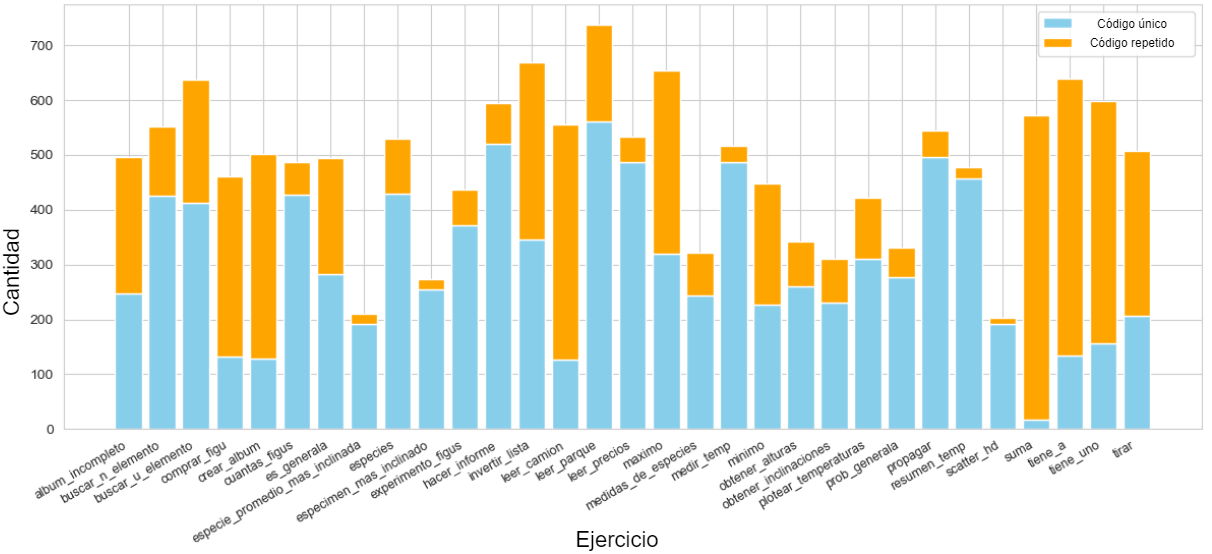
\includegraphics[width=\linewidth]{imagenes/unique-1.png}
        \caption{Cantidad total de código repetido y de código único por ejercicio}
        \label{fig:figura1}
    \end{subfigure}
    \hfill
    \begin{subfigure}{0.45\textwidth}
        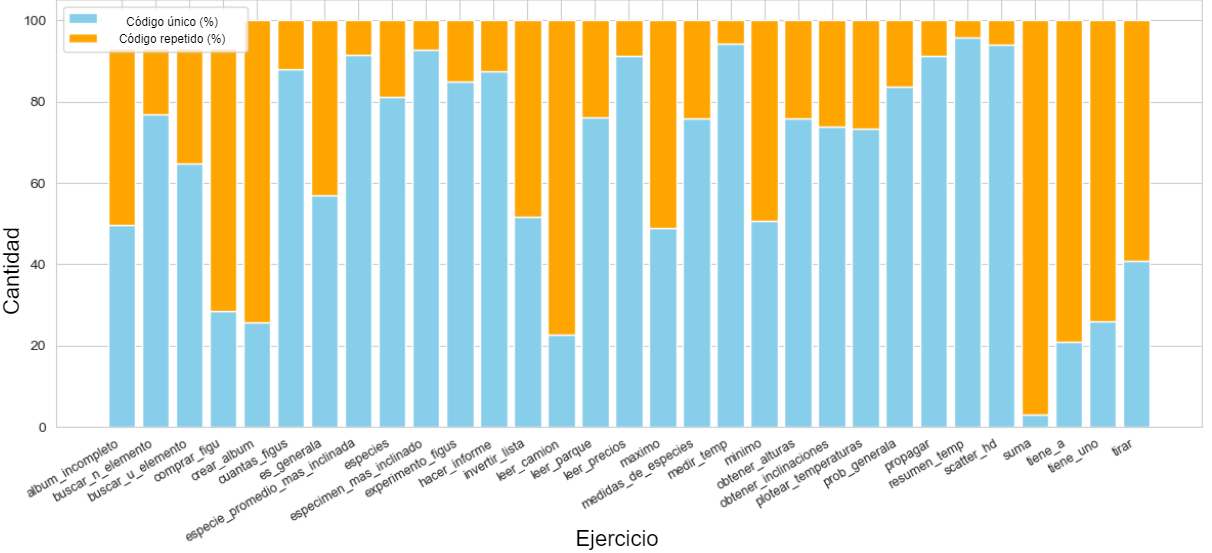
\includegraphics[width=\linewidth]{imagenes/unique-2.png}
        \caption{Proporción de código repetido y de código único por ejercicio}
        \label{fig:figura2}
    \end{subfigure}
    \caption{Código repetido a lo largo de los 31 entregables, ordenados por orden cronológico.}
    \label{fig:figuras_juntas}
\end{figure}

Como es de esperarse, en ejercicios más introductorios la proporción de código idéntico es mayor. Esto podría deberse a la simpleza del funcionamiento esperado de dichas funciones (como, por ejemplo, en el caso \emph{suma}).

A continuación, se realizó un \emph{mapeo} entre alumnos con código idéntico y el programa en cuestión. Una vez realizado esto, se generó un nuevo \emph{dataset} sin dichas producciones. Se realizó entonces el procedimiento similar anterior: Reducción de la dimensionalidad de los datos con códigos únicos usando PCA $\rightarrow$ Aplicación de \emph{Kmeans} $\rightarrow$ Re-inclusión de los alumnos que habían sido \emph{mapeados} y eliminados anteriormente.

\begin{figure}[H]
    \centering
    \begin{subfigure}{0.45\textwidth}
        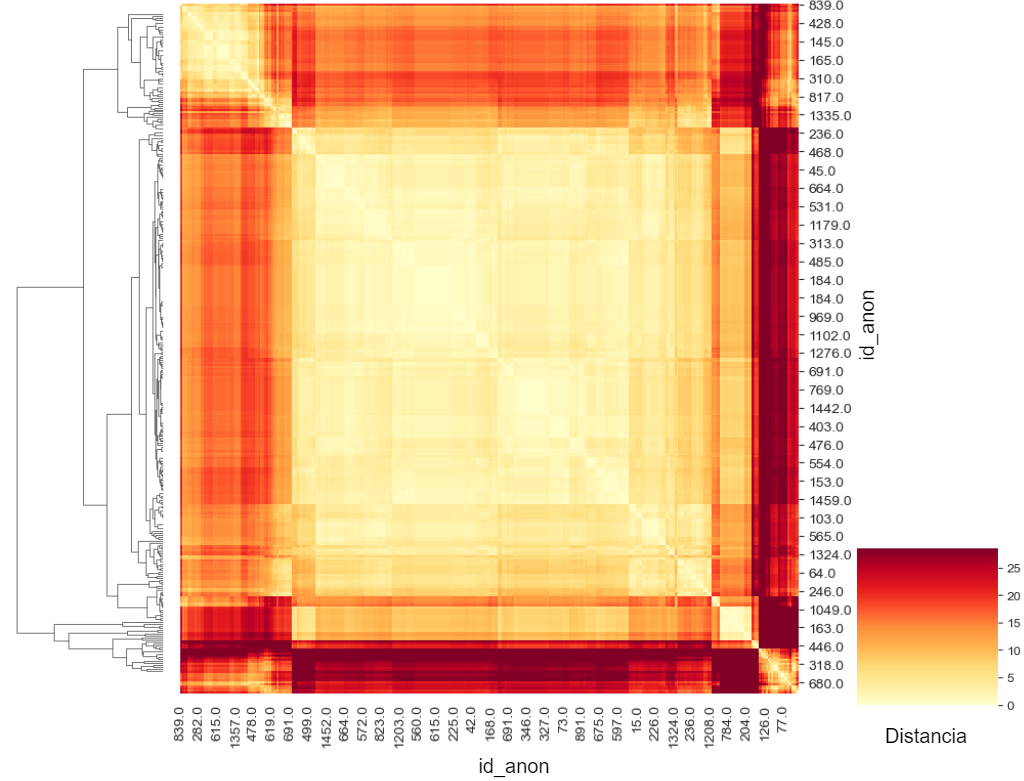
\includegraphics[width=\linewidth]{imagenes/codigo-reptido-original.png}
        \caption{Datos originales.}
        \label{fig:figura3}
    \end{subfigure}
    \hfill
    \begin{subfigure}{0.45\textwidth}
        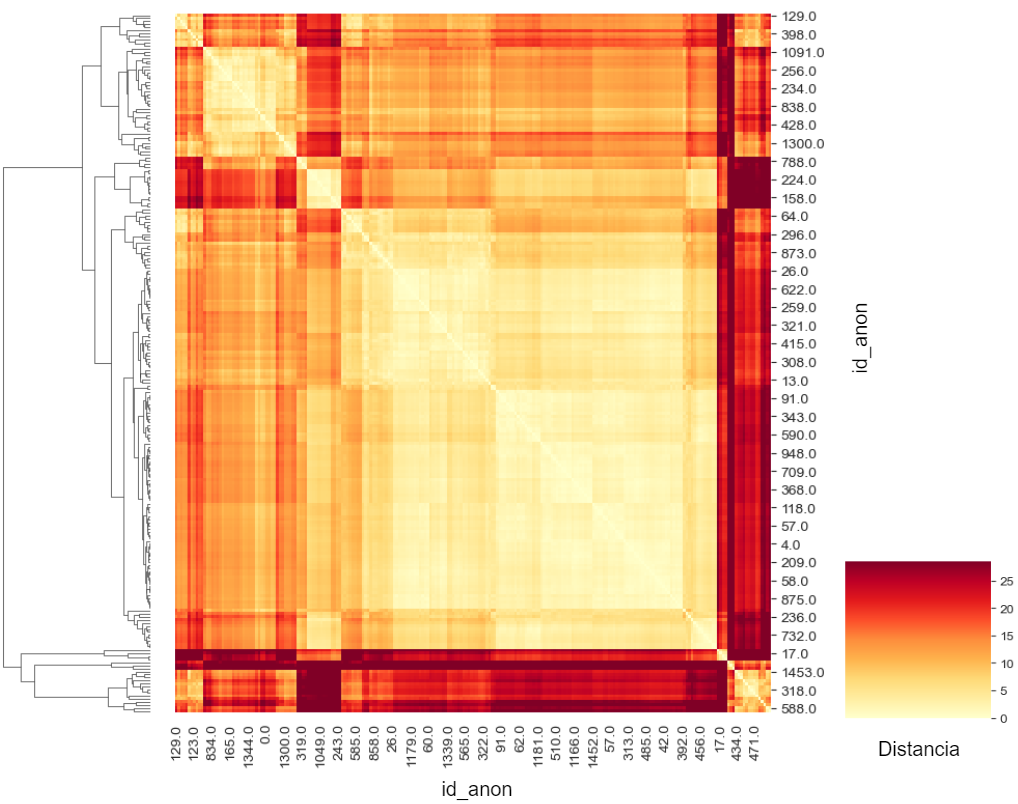
\includegraphics[width=\linewidth]{imagenes/codigo-reptido-uniques.png}
        \caption{Datos sin código repetido.}
        \label{fig:figura4}
    \end{subfigure}
    \caption{\emph{Heatmaps} para el ejercicio \emph{obtener\_inclinaciones} de la unidad tres con el agrupamiento realizado con los datos originales y con los datos sin el código repetido.}
    \label{fig:figuras_juntas}
\end{figure}

Como se observa en la figura anterior, a modo de ejemplo, no se observó una diferencia significativa entre el \emph{clustering} original y aquél realizado contemplando lo mencionado anteriormente para ninguno de los 31 ejercicios.

Como última medida, se observó la proporción \emph{cluster} a \emph{cluster} de alumnos que habían finalizado el curso, esperando ver una diferencia significativa:

\begin{figure}[H]
    \centering
    \begin{subfigure}{0.45\textwidth}
        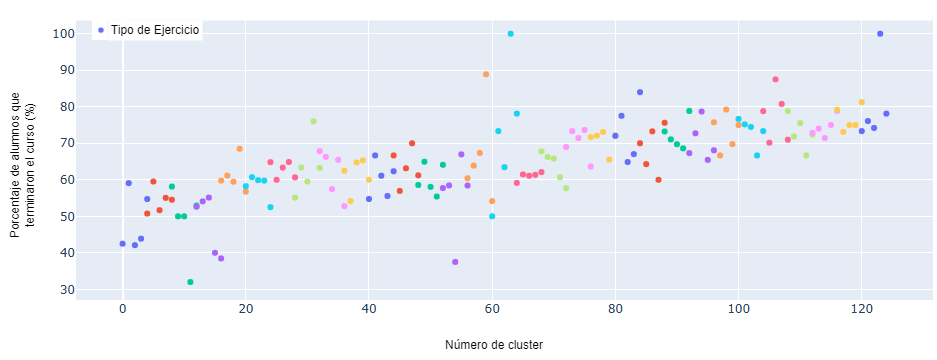
\includegraphics[width=\linewidth]{imagenes/porcentaje - original.png}
        \caption{Datos originales.}
        \label{fig:figura5}
    \end{subfigure}
    \hfill
    \begin{subfigure}{0.45\textwidth}
        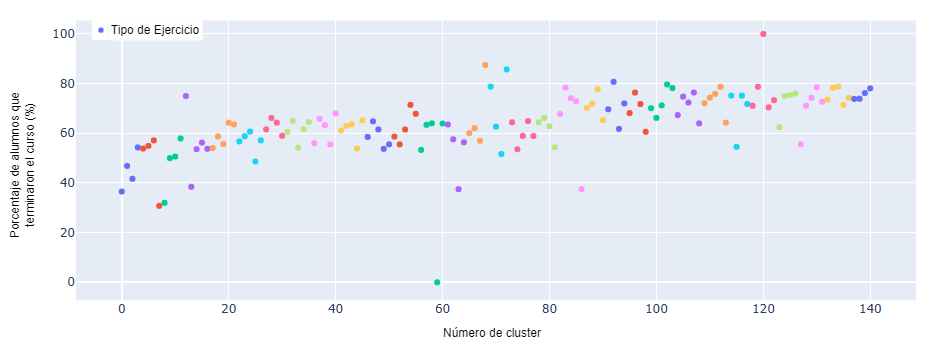
\includegraphics[width=\linewidth]{imagenes/porcentaje - unniques.png}
        \caption{Datos sin código repetido.}
        \label{fig:figura6}
    \end{subfigure}
    \caption{Comparación entre el porcentaje de alumnos que finalizaron el curso \emph{cluster} a \emph{cluster} para los datos originales y los datos después de haber \emph{mapeado} el código repetido.}
    \label{porcentajes}
\end{figure}

Hubiera sido deseable observar que las diferencias entre dichas proporciones para cada ejercicio estuvieran más marcadas. Por el contrario, parecería haber una mejor separación de los dos grupos utilizando los datos originales.

Luego, no parecería haber un indicador de que el código idéntico incida sobre la \emph{clusterización} de los alumnos.


\subsection{Inserción de datos de interés}
Para esta sección se le intentó hacer foco a ciertas características del código producido por los estudiantes, cuya extracción se comentó en la Sección~\ref{subsec:extraccion}. Se hizo un particular hincapié en el número de líneas, agregándolo como una nueva componente tanto en el vector de \emph{embeddings} como luego de su reducción de la dimensionalidad. En ninguno de los dos casos se observaron cambios significativos en el agrupamiento. Una posible explicación es que el modelo ya contempla estas características inherentes al código en cuestión, por lo que no parecería estar incorporándose información adicional. 


\subsection{Usando \emph{embeddings} normalizados}
Se realizó nuevamente un análisis análogo al de la Figura \ref{cluster}, obteniéndose los siguientes resultados:

\begin{figure}[H]
    \centering
    \includegraphics[width=0.5\textwidth]{imagenes/cluster-normalized.png}
    \caption{Cantidad de \emph{clusters} compartidos por estudiante con \emph{embeddings} con normalizados.}
\end{figure}

Esto no agregó información adicional por sobre lo realizado anteriormente. Tras haber replicado el procedimiento de los \emph{cliques}, estos retornaron resultados muy similares a los anteriores, teniendo como diferencia apenas un par de estudiantes por grupo. 



\subsection{Fuzzy-2-means}

Una característica útil de \emph{Fuzzy-2-means} es que este permite que algunos puntos pertenezcan \emph{parcialmente} a un grupo. En pos de distinguir entre aquellos estudiantes que habían finalizado el curso y a los que habían continuado más allá del primer parcial pero sin terminar la materia, se aplicó \emph{Fuzzy-2-means} a los datos originales: 

\begin{figure}[H]
    \centering
    \begin{subfigure}{0.45\textwidth}
        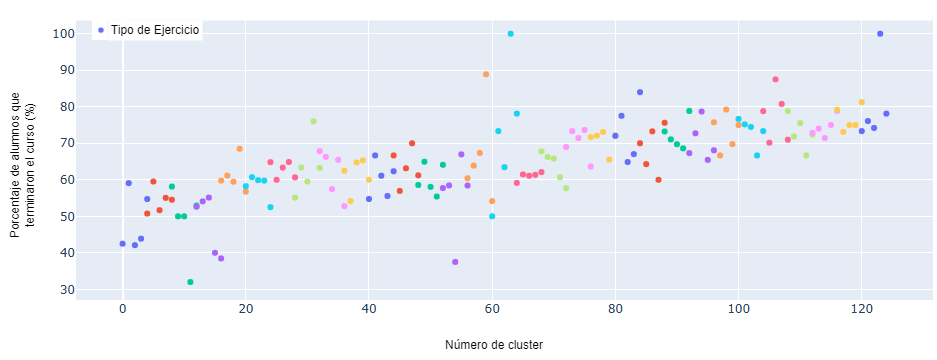
\includegraphics[width=\linewidth]{imagenes/porcentaje - original.png}
        \caption{Datos originales con \emph{Kmeans}.}
        \label{fig:figura5}
    \end{subfigure}
    \hfill
    \begin{subfigure}{0.45\textwidth}
        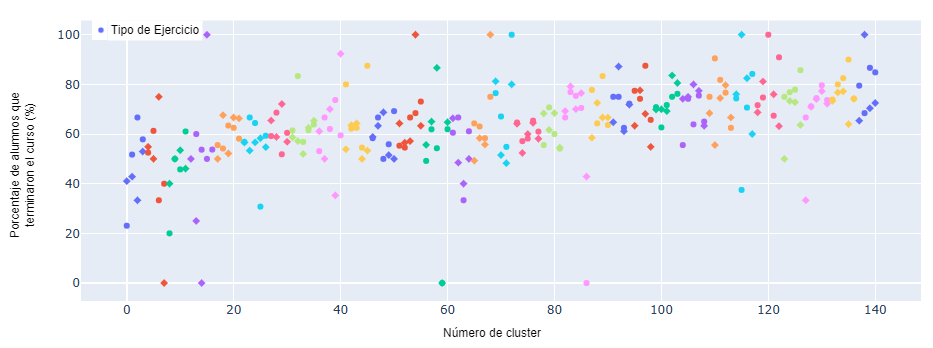
\includegraphics[width=\linewidth]{imagenes/porcentaje - fuzzy.png}
        \caption{Datos originales con \emph{Fuzzy-2-means}.}
        \label{fig:figura6}
    \end{subfigure}
    \caption{Comparación entre el porcentaje de alumnos que finalizaron el curso \emph{cluster} a \emph{cluster} para los datos originales con distintos algoritmos de agrupación.}
    \label{porcentajes}
\end{figure}

No se observaron alumnos a los cuales asignara parcialmente a un grupo, perteneciendo todos en su totalidad a alguno de los \emph{clusters} mostrados en la figura anterior. Si se observó un incremento en la cantidad de \emph{clusters} que, si bien son más homogéneos, se debe a que estos son muy pequeños, contando con una cantidad de apenas algunos estudiantes. Luego, este algoritmo no proporcionó información adicional por sobre el \emph{Kmeans} tradicional, para este caso particular.

\section{Representando a los alumnos como un único vector}

Teniendo en cuenta resultados anteriores, se consideraron los vectores generados por el modelo \emph{CodeBERT} y se los concatenó respetando el el orden cronológico del curso, obeteniendo así un único vector por estudiante. Con esto se esperaba poder distinguir de mejor manera a quienes habían terminado el curso de quienes no. Más específico aún, a quienes lo finalizaron de quienes lo continuaron después del primer examen.


\subsection{Vectores de ceros}

Es deseable que los vectores de cada estudiante posean la misma dimensión, para así poder replicar el procedimiento descrito en secciones anteriores de reducción de dimensionalidad y agrupamiento. Un desafío a la hora de encarar este enfoque fue el ``rellenado'' de las entregas no realizadas por los alumnos.

 En un primer intento, para cada individuo y, para cada ejercicio, se concatenaron:

 \begin{itemize}
     \item Con el \emph{embedding} correspondiente a la entrega, de estar presente.
     \item Con un vector de 768 ceros (dimensión del \emph{output} de \emph{CodeBERT}).
 \end{itemize}

\begin{figure}[H]
    \centering
    \includegraphics[width=\textwidth]{imagenes/fill functiontodos_los_graficos_en_una_sola_figura.png}
    \caption{Resultado de realizar PCA y \emph{Kmeans} con \emph{k} = 2 con cada estudiante representando un único vector; agregando de a un ejercicio por vez. Ejercicios no entregados rellenados con vectores nulos.}
    \label{fig: zeros}
\end{figure}

\subsection{Función vacía}
Si bien el enfoque anterior parece razonable, es muy difícil saber qué representa un vector de ceros en el dominio de \emph{CodeBERT}. Luego, se decidió repetir el procedimiento anterior, ahora rellenando con una ``función vacía''. Entonces obtuvimos, para cada alumno una concatenación:


 \begin{itemize}
     \item Con el \emph{embedding} correspondiente a la entrega, de estar presente.
     \item Con un vector representando la ``función vacía'' para ese ejercicio. A modo de ejemplo, para el ejercicio \emph{buscar\_u\_elemento}, obtendríamos los \emph{embeddings} de la siguiente producción:
 \end{itemize}


\begin{lstlisting}[style=pythonstyle]
def buscar_u_elemento():
    pass
\end{lstlisting}

Obteniéndose el siguiente resultado:

\begin{figure}[H]
    \centering
    \includegraphics[width=\textwidth]{imagenes/zerostodos_los_graficos_en_una_sola_figura.png}
    \caption{Resultado de realizar PCA y \emph{Kmeans} con \emph{k} = 2 con cada estudiante representando un único vector; agregando de a un ejercicio por vez. Ejercicios no entregados rellenados con el vector correspondiente a la función vacía}
    \label{fig: fill func}
\end{figure}

\subsection{Comparación respecto a la proporción de entregas}

Para evaluar la incidencia de la añadidura de vectores sintéticos en los \emph{embeddings} concatenados de los estudiantes, se analizó la cantidad de entregas total por ejercicio.  

\begin{figure}[H]
    \centering
    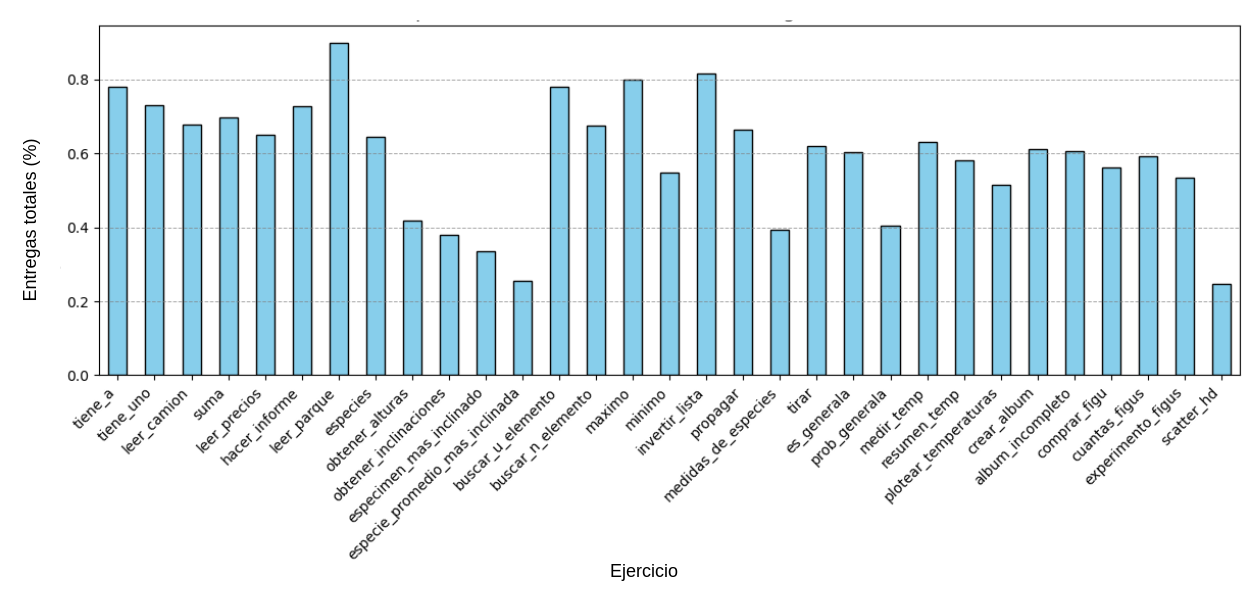
\includegraphics[width=\textwidth]{imagenes/proporcion - entregas (1).png}
    \caption{Proporción de estudiantes que entregaron cada ejercicio.}
\end{figure}

Se observó que la información proporcionada por la Figura anterior y las Figuras \ref{fig: zeros} y \ref{fig: fill func}, era muy similar: si bien para el ejercicio \emph{experimento\_figus} en el \emph{cluster\_0} podemos observar que, la cantidad de los estudiantes que luego finalizaron el curso es del 74\%, si nos focalizamos únicamente en los alumnos que efectivamente entregaron este ejercicio, en este grupo se encuentra un 80\% de los estudiantes que lo terminaron. 

Mientras que, en instancias más preliminares, los resultados del \emph{clustering} en cuanto a proporciones de estos dos grupos se sostienen cercanas al 50\%, por lo que tampoco resultan de utilidad. Luego, podríamos decir que hay indicadores de que para este caso y por cómo fueron los vectores individuales, el agrupamiento separa por entregas realizadas y no por quiénes finalizarán el curso.

\chapter{Conclusión}

Este trabajo abordó el análisis del comportamiento estudiantil en un curso Introductorio a Python en contexto de pandemia, centrándose exclusivamente en el análisis de las producciones de código de los alumnos. El objetivo principal fue identificar patrones que permitieran detectar grupos con mayor propensión a la deserción.

El \emph{dataset} analizado comprende las entregas de 819 estudiantes a lo largo del curso, considerando únicamente la última versión de cada ejercicio como producción definitiva. El preprocesamiento de los datos incluyó la anonimización del código, para preservar la privacidad del alumnado, y la limpieza de los datos, que permitió eliminar entregas incorrectas y reducir la cantidad de código no procesable por el modelo. Para garantizar la seguridad de esta información sensible, se implementó una base de datos \emph{local} que permitió el almacenamiento y procesamiento seguro de los datos.

En un primer análisis, se realizó un estudio detallado de las entregas examinando cada ejercicio de manera individual. Si bien se identificaron grupos claramente definidos para algunos ejercicios, no se encontró una correlación significativa entre estos patrones de agrupamiento y las variables objetivo de predicción. Esta falta de asociación sugiere que las características que definen los grupos no necesariamente están alineadas con los indicadores de rendimiento que se buscaba predecir.

En un segundo análisis, se realizó una comparación exhaustiva entre todos los \emph{clusters} generados a lo largo del curso. Los resultados revelaron valores bajos tanto en los índices ARI (\emph{Adjusted Rand Index}) como NMI (\emph{Normalized Mutual Information}). De manera similar, los índices de Jaccard también mostraron valores reducidos. Estos resultados, en conjunto, sugieren una baja similitud estructural entre las diferentes particiones generadas, indicando que los patrones de agrupamiento varían significativamente entre las distintas etapas del curso.

En un tercer análisis, se examinó la distribución de \emph{clusters} compartidos por cada estudiante. Durante esta exploración, se identificó un grupo de particular interés: aquellos estudiantes que compartían 13 o más \emph{clusters} a lo largo del curso. Un análisis posterior reveló hallazgos significativos sobre este conjunto. No solo representaba más de la mitad de los estudiantes que eventualmente abandonarían la materia, sino que, más específicamente, englobaba a aquellos que la abandonarían después de la primera instancia de evaluación. Esta observación sugiere un patrón de comportamiento distintivo que podría servir como indicador temprano de deserción.

Se implementaron diversos enfoques con el objetivo de mejorar la distinción entre dos grupos de estudiantes: aquellos que completaron el curso y aquellos que mantuvieron su participación, al menos, hasta la quinta unidad incluida en este \emph{dataset}. Las estrategias exploradas incluyeron: (i) el análisis de la incidencia del código repetido en la \emph{clusterización}, (ii) la incorporación de información adicional relevante, (iii) la normalización de los \emph{embeddings}, y (iv) la implementación de una variante del algoritmo \emph{K-means} para el agrupamiento. Sin embargo, ninguna de estas aproximaciones resultó en mejoras significativas respecto a los resultados previamente obtenidos.

Finalmente, se adoptó un enfoque alternativo donde cada estudiante fue representado como un único vector. Para abordar los ejercicios no entregados, se exploraron dos estrategias de completado de datos: inicialmente se utilizaron vectores nulos (de ceros) y posteriormente se implementó el \emph{embedding} correspondiente a la función vacía. Ambos enfoques retornaron resultados similares; sin embargo, tanto la reducción de dimensionalidad como la \emph{clusterización} resultante reflejaron principalmente patrones relacionados con la cantidad de entregas realizadas por cada estudiante, en lugar de identificar efectivamente a quienes completarían el curso. Esta observación sugiere que la representación vectorial propuesta capturó más la frecuencia de participación que los indicadores de éxito académico.

Los resultados obtenidos sugieren que, si bien el análisis del código por sí solo no fue suficiente para predecir con precisión la finalización del curso, permitió identificar patrones de comportamiento tempranos potencialmente indicativos de deserción, particularmente en estudiantes que comparten características de agrupamiento específicas después de la primera evaluación. Este hallazgo podría ser valioso para el desarrollo de estrategias de intervención temprana en futuros cursos.

\chapter{Trabajo futuro}

Mencionan Cerdeiro et al. que para llevar a cabo el curso en pandemia se utilizaron distintos canales de difusión y comunicación como Slack, lo que permitió que las \emph{... consultas estuvieran ordenadas de manera tal que otros estudiantes pudieran buscar y revisarlas fácilmente, aprovecharlas, incluso comentar sobre ellas, lo que evitó que se repitieran las consultas} \cite{unsam2020}. En ``Embedding navigation patterns for student performance prediction'', Loginova et al. buscaron predecir el rendimiento académico de los estudiantes utilizando patrones de navegación en una plataforma educativa en línea, en lugar de basarse en calificaciones anteriores \cite{loginova2021embedding}. En este estudio mencionan que el análisis de las secuencias de acciones de los estudiantes a lo largo de un curso permitieron identificar estrategias de aprendizaje distintas entre estudiantes de alto y bajo rendimiento, siendo útiles para sistemas de alerta temprana. Basándonos entonces en esta última propuesta, en un futuro quizás podría explorarse la posibilidad de intentar diferenciar a los alumnos que finalizarán el curso de los que no (pero completaron gran parte del mismo) basándonos no solamente en el código sino también en interacciones como la previamente mencionada. 

Sería interesante y sencillo, por cómo la base de datos fue generada, también considerar como información adicional la cantidad de entregas por alumno. En un futuro podía hacerse un análisis más exhaustivo por alumno, considerando no solamente su trayectoria ejercicio a ejercicio sino además dentro de cada entrega. 

Podríamos además explorar no solamente quiénes finalizarán el curso para un trabajo futuro sino además intentar estimar cuántos alumnos se presentarán a los parciales. Podríamos analizar si además de dejar de entregar depués de la primera evaluación, el grupo que compartía más de 13 \emph{clusters} se llegó a presentar. Esto podría resultar particularmente útil para docentes en su organización de la materia y tiempos de corrección. 
%%%% BIBLIOGRAFIA
\backmatter
\bibliographystyle{unsrt}
\bibliography{tesis}

\end{document}
